\documentclass{article}
\usepackage{etex}
\usepackage[T1]{fontenc}
\usepackage[bitstream-charter]{mathdesign}
\usepackage[scaled=0.92]{PTSans}
\renewcommand*\ttdefault{lmvtt}
\usepackage{exscale}

\usepackage[final,expansion=alltext]{microtype}
\usepackage[english]{babel}
\usepackage{ragged2e}

\usepackage{amsmath}
\usepackage{graphicx}                               % graphics
\usepackage{booktabs, array}                        % nice tables
\usepackage[algoruled]{algorithm2e}                 % pseudocode
\usepackage[numbers,sort]{natbib}                   % better bibliography
\usepackage{cleveref}                               % the best package ever
\usepackage[acronym,smallcaps,nowarn]{glossaries}   % second best package ever

% COLORS
\newcommand{\gray}[1]{\textcolor{black!60}{#1}}
\newcommand{\blu}[1]{\textcolor{jblue}{#1}}

\newacronym{ELBO}{elbo}{evidence lower bound}
\newacronym{KL}{kl}{Kullback-Leibler}

\newacronym{DEF}{def}{deep exponential family}
\newacronym{DLGM}{dlgm}{deep latent Gaussian model}
\newacronym{DRAW}{draw}{Deep Recurrent Attentive Writer}

\newacronym{MF}{mf}{mean-field}
\newacronym{VGP}{vgp}{variational Gaussian process}
\newacronym{BBVI}{bbvi}{black box variational inference}
\newacronym{ADVI}{advi}{automatic differentiation variational inference}
\newacronym{NF}{nf}{normalizing flows}
\newacronym{CVI}{cvi}{copula variational inference}
\newacronym{VAE}{vae}{variational autoencoder}
\newacronym{IWAE}{iwae}{importance weighted autoencoder}
\newacronym{NVIL}{nvil}{neural variational inference}
\newacronym{MIXTURE}{mixture}{}
\newacronym{DSVI}{dsvi}{}

\newacronym{VI}{vi}{variational inference}
\newacronym{EP}{ep}{expectation propagation}

\newacronym{LS}{ls}{Langevin-Stein}
\newacronym{OPVI}{opvi}{operator variational inference}

\DeclareRobustCommand{\mb}[1]{\ensuremath{\boldsymbol{\mathbf{#1}}}}
\DeclareRobustCommand{\mbf}[1]{\ensuremath{\textbf{#1}}}
\DeclareMathOperator*{\argmax}{arg\,max}
\DeclareMathOperator*{\argmin}{arg\,min}


\newcommand{\KL}[2]{\ensuremath{\textrm{KL}\left(#1\;\|\;#2\right)}}

\renewcommand{\mid}{~\vert~}

\newcommand{\mbw}{\mb{w}}
\newcommand{\mbW}{\mb{W}}

\newcommand{\mbx}{\mb{x}}
\newcommand{\mbX}{\mbf{X}}

\newcommand{\mby}{\mb{y}}
\newcommand{\mbY}{\mbf{Y}}

\newcommand{\mbz}{\mb{z}}
\newcommand{\mbZ}{\mb{Z}}

\newcommand{\mbI}{\mbf{I}}
\newcommand{\mbone}{\mbf{1}}

\newcommand{\mbL}{\mbf{L}}

\newcommand{\mbtheta}{\mb{\theta}}
\newcommand{\mbTheta}{\mb{\Theta}}
\newcommand{\mbomega}{\mb{\omega}}
\newcommand{\mbOmega}{\mb{\Omega}}
\newcommand{\mbsigma}{\mb{\sigma}}
\newcommand{\mbSigma}{\mb{\Sigma}}
\newcommand{\mbphi}{\mb{\phi}}
\newcommand{\mbPhi}{\boldsymbol{\Phi}}
% \newcommand{\mblambda}{\mb{\lambda}}

\newcommand{\mbalpha}{\mb{\alpha}}
\newcommand{\mbbeta}{\mb{\beta}}
\newcommand{\mbgamma}{\mb{\gamma}}
\newcommand{\mbeta}{\mb{\eta}}
\newcommand{\mbmu}{\mb{\mu}}
\newcommand{\mbrho}{\mb{\rho}}
\newcommand{\mblambda}{\mb{\lambda}}
\newcommand{\mbzeta}{\mb{\zeta}}

\newcommand\dif{\mathop{}\!\mathrm{d}}
\newcommand{\diag}{\textrm{diag}}
\newcommand{\supp}{\textrm{supp}}

\newcommand{\E}{\mathbb{E}}
\newcommand{\bbH}{\mathbb{H}}
\newcommand{\Var}{\mathbb{V}\textrm{ar}}

\newcommand{\bbN}{\mathbb{N}}
\newcommand{\bbZ}{\mathbb{Z}}
\newcommand{\bbR}{\mathbb{R}}
\newcommand{\bbS}{\mathbb{S}}

\newcommand{\cL}{\mathcal{L}}

\newcommand{\cN}{\mathcal{N}}
\newcommand{\cT}{\mathcal{T}}
\newcommand{\Gam}{\textrm{Gam}}
\newcommand{\InvGam}{\textrm{InvGam}}

\usepackage{tikz}
\usetikzlibrary{bayesnet}

\pgfdeclarelayer{edgelayer}
\pgfdeclarelayer{nodelayer}
\pgfsetlayers{edgelayer,nodelayer,main}

\definecolor{hexcolor0xbfbfbf}{rgb}{0.749,0.749,0.749}

\tikzset{>=latex}
\tikzstyle{none}   = [inner sep=0pt]
\tikzstyle{line}   = [-,
                      thick,
                      shorten <=1pt,
                      shorten >=1pt]
\tikzstyle{arrow}  = [->,
                      thick,
                      shorten <=1pt,
                      shorten >=1pt]
\tikzstyle{ardash} = [dashed,
                      ->,
                      thick,
                      shorten <=1pt,
                      shorten >=1pt]

\tikzstyle{empty}=[
                   circle,
                   opacity=0.0,
                   text opacity=1.0,
                   inner sep=0pt
                  ]

\tikzstyle{box}=[
                 rectangle,
                 fill=White,
                 thick,
                 draw=Black,
                 inner sep=7pt
                ]

\tikzstyle{filled}=[
                    circle,
                    thick,
                    fill=hexcolor0xbfbfbf,
                    draw=Black
                   ]

\tikzstyle{hollow}=[
                    circle,
                    thick,
                    fill=White,
                    draw=Black
                   ]

\tikzstyle{param}=[
                   rectangle,
                   fill=Black,
                   draw=Black,
                   inner sep=0pt,
                   minimum width=4pt,
                   minimum height=4pt
                  ]

\tikzstyle{paramhollow}=[
                         rectangle,
                         thick,
                         fill=White,
                         draw=Black,
                         inner sep=0pt,
                         minimum
                         width=4pt,
                         minimum height=4pt
                        ]

\usepackage{pgfplots}                               % PGFPLOTS baby!
\pgfplotsset{compat=newest}
\pgfplotsset{plot coordinates/math parser=false}
% \usepgfplotslibrary{statistics}


\title{
Edward: A library for probabilistic modeling,\break inference, and criticism
}

\author{
Dustin Tran, Alp Kucukelbir, Adji B.~Dieng,\\
Maja Rudolph, Dawen Liang, and David M.~Blei\\\\
Columbia University
}

\begin{document}

\hypersetup{pageanchor=false}
\begin{titlepage}
\maketitle
\begin{abstract}
  Probabilistic modeling is a powerful approach for analyzing
  empirical information.
  We describe \emph{Edward}, a library for probabilistic modeling.
  Edward's design reflects an iterative process pioneered by George
  Box: build a model of a phenomenon, make inferences about the model given
  data, and criticize the model's fit to the data. Edward supports a broad class
  of probabilistic models, efficient algorithms for inference, and many
  techniques for model criticism. The library builds on top of
  TensorFlow to support distributed training and hardware such as
  GPUs.
  Edward enables the development of complex probabilistic
  models and their algorithms at a massive scale.
\end{abstract}

\emph{Keywords:}
Probabilistic Models;
Bayesian Inference;
Model Criticism;
Neural Networks;
Scalable Computation;
Probabilistic Programming.%
\footnote{Details in this paper describe Edward version 1.2.1,
released Jan 30, 2017.}

\setcounter{secnumdepth}{2}
\setcounter{tocdepth}{2}
\tableofcontents

\thispagestyle{empty}
\end{titlepage}
\hypersetup{pageanchor=true}

\glsresetall{}

\clearpage

\vspace{-1.0ex}
\section{Introduction}
\label{sec:introduction}
\vspace{-0.5ex}
The nature of deep neural networks is compositional. Users can connect
layers in creative ways, without having to worry about how to perform
testing (forward propagation) or inference (gradient-based
optimization, with back propagation and automatic differentiation).

In this paper, we design compositional representations for
probabilistic programming.  Probabilistic programming lets users
specify generative probabilistic models as programs and then
``compile'' those models down into inference procedures.
Probabilistic models are also compositional in nature, and much work
has enabled rich probabilistic programs via compositions of random
variables
\citep{goodman2012church,ghahramani2015probabilistic,lake2016building}.

Less work, however, has considered an analogous compositionality for
inference. Rather, many existing \glsreset{PPL}\acrlongpl{PPL} treat
the inference engine as a black box, abstracted away from the model.
These cannot capture probabilistic inferences that
reuse the model's representation---a key idea in
recent advances in variational
inference~\citep{kingma2014autoencoding,rezende2015variational,tran2016variational},
\glsreset{GAN}\acrlongpl{GAN}~\citep{goodfellow2014generative},
and also in more classic inferences
\citep{dayan1995helmholtz,gutmann2010noise}.

We propose Edward\footnote{%
  See \citet{tran2016edward}
  for details of the API. A companion webpage for this paper is available at
  \url{http://edwardlib.org/iclr2017}. It contains more complete
  examples with runnable code.}, a
Turing-complete \acrlong{PPL} which builds on two compositional
representations---one for random variables and one for inference.
By treating inference as a first class citizen, on a
par with modeling, we show that probabilistic programming can be as
flexible and computationally efficient as traditional deep learning.
For flexibility, we show how Edward makes it easy to fit
the same model using a variety of composable inference methods,
ranging from point estimation to variational inference to
\acrshort{MCMC}.
For efficiency, we
show how to integrate Edward into existing computational graph
frameworks such as TensorFlow \citep{abadi2016tensorflow}.  Frameworks
like TensorFlow provide computational benefits like distributed
training, parallelism, vectorization, and \glsunset{GPU}\gls{GPU}
support ``for free.''
For example, we show on a benchmark task that Edward's
\acrlong{HMC} is many times faster than existing software. Further, Edward
incurs no runtime overhead: it is as fast as handwritten TensorFlow.

%%% Local Variables:
%%% mode: latex
%%% TeX-master: "main"
%%% End:

\subsection*{Related work}

\textbf{Probabilistic programming.}
There has been much work on programming languages which specify
broad classes of probabilistic models, or probabilistic
programs. Recent works include
Church \citep{goodman2012church},
Venture \citep{mansinghka2014venture},
Anglican \citep{wood2015new},
Stan \citep{carpenter2016stan}, and
WebPPL \citep{goodman2014design}.
The most important distinction in Edward stems from motivation. We
are interested in deploying probabilistic models to many real
world applications, ranging from the size of data and data structure,
such as large text corpora or many brief audio signals, to the size of
model and class of models, such as small nonparametric models or deep
generative models. Thus Edward is built with fast computation in
mind.

\textbf{Black box inference.}
Black box algorithms are typically based on Monte Carlo methods, and
make very few assumptions about the
model \citep{metropolis1949monte,hastings1970monte,geman1984stochastic}.
Our motivation as outlined
above presents a new set of challenges in both inference research and
software design. As a first consequence, we focus on variational
inference \citep{hinton1993keeping,waterhouse1996bayesian,jordan1999introduction}.
As a second consequence, we encourage active research on
inference by providing a class hierarchy of inference algorithms. As a
third consequence, our inference algorithms aim to take advantage of
as much structure as possible from the model. Edward supports all
types of inference, whether they
be black box or model-specific \citep{dempster1977em,hoffman2013stochastic}.

\textbf{Computational frameworks.}
There are many computational frameworks, primarily built for deep
learning: as of this date, this includes
TensorFlow \citep{abadi2016tensorflow},
Theano \citep{alrfou2016theano},
Torch \citep{collobert2011torch7},
neon \citep{nervana2014neon}, and
the Stan Math Library \citep{carpenter2015stan}.
These are incredible tools which Edward employs as a backend. In terms
of abstraction, Edward sits one level higher.

\textbf{High-level deep learning libraries.}
Neural network libraries such as
Keras \citep{chollet2015keras} and
Lasagne \citep{lasagne}
are at a similar abstraction level as Edward. However both are primarily
interested in parameterizing complicated functions for supervised
learning on large datasets. We are interested in probabilistic models
which apply to a wide array of learning tasks. These tasks may have both
complicated likelihood and complicated priors (neural networks are an
option but not a necessity). Therefore our goals are orthogonal and in
fact mutually beneficial to each other. For example, we use Keras'
abstraction as a way to easily specify models parameterized by deep
neural networks.

\clearpage
\section{Getting Started}
\label{sec:getting-started}

Probabilistic modeling in Edward uses a simple language of
random variables.
Here we will show a Bayesian neural network. It is a neural network
with a prior distribution on its weights.

First, simulate a toy dataset of 50 observations with a cosine relationship.

\begin{lstlisting}
import numpy as np

x_train = np.linspace(-3, 3, num=50)
y_train = np.cos(x_train) + np.random.normal(0, 0.1, size=50)
x_train = x_train.astype(np.float32).reshape((50, 1))
y_train = y_train.astype(np.float32).reshape((50, 1))
\end{lstlisting}

\begin{figure}[h]
\centering
\includegraphics[width=3.5in]{images/getting-started-fig0.pdf}
\caption{Simulated data with a cosine relationship between $x$ and $y$.}
\end{figure}

Next, define a two-layer Bayesian neural network. Here, we
define the neural network manually with \texttt{tanh} nonlinearities.

\begin{lstlisting}[language=Python]
import tensorflow as tf
from edward.models import Normal

W_0 = Normal(mu=tf.zeros([1, 2]), sigma=tf.ones([1, 2]))
W_1 = Normal(mu=tf.zeros([2, 1]), sigma=tf.ones([2, 1]))
b_0 = Normal(mu=tf.zeros(2), sigma=tf.ones(2))
b_1 = Normal(mu=tf.zeros(1), sigma=tf.ones(1))

x = x_train
y = Normal(mu=tf.matmul(tf.tanh(tf.matmul(x, W_0) + b_0), W_1) + b_1,
           sigma=0.1)
\end{lstlisting}

Next, make inferences about the model from data. We will use variational
inference. Specify a normal approximation over the weights and biases.

\begin{lstlisting}[language=Python]
qW_0 = Normal(mu=tf.Variable(tf.zeros([1, 2])),
              sigma=tf.nn.softplus(tf.Variable(tf.zeros([1, 2]))))
qW_1 = Normal(mu=tf.Variable(tf.zeros([2, 1])),
              sigma=tf.nn.softplus(tf.Variable(tf.zeros([2, 1]))))
qb_0 = Normal(mu=tf.Variable(tf.zeros(2)),
              sigma=tf.nn.softplus(tf.Variable(tf.zeros(2))))
qb_1 = Normal(mu=tf.Variable(tf.zeros(1)),
              sigma=tf.nn.softplus(tf.Variable(tf.zeros(1))))
\end{lstlisting}

Defining \texttt{tf.Variable} allows the variational factors'
parameters to vary. They are all initialized at 0. The standard
deviation parameters are constrained to be greater than zero according
to a
softplus transformation\footnote{
The softplus function is defined as $\textrm{softplus}(x) =
\log(1+\exp(x))$.}.

Now, run variational inference with the
Kullback-Leibler divergence
in order to infer the model's latent variables given data.
We specify \texttt{1000} iterations.

\begin{lstlisting}[language=Python]
import edward as ed

inference = ed.KLqp({W_0: qW_0, b_0: qb_0,
                     W_1: qW_1, b_1: qb_1}, data={y: y_train})
inference.run(n_iter=1000)
\end{lstlisting}

Finally, criticize the model fit. Bayesian neural networks define a distribution
over neural networks, so we can perform a graphical check. Draw neural networks
from the inferred model and visualize how well it fits the data.

\begin{figure}[h]
\centering
\includegraphics[width=3.5in]{images/getting-started-fig1.pdf}
\caption{Posterior draws from the inferred Bayesian neural network.}
\end{figure}

The model has captured the cosine relationship between $x$ and $y$
in the observed domain.

\clearpage
\section{Design}
\label{sec:design}

Edward's design reflects the building blocks for probabilistic
modeling. It defines interchangeable components, enabling rapid
experimentation and research with probabilistic models.

Edward is named after the innovative statistician
George Edward Pelham Box. Edward follows Box's philosophy of statistics and
machine learning \citep{box1976science}.

First gather data from some real-world phenomena. Then cycle through
Box's loop \citep{blei2014build}.

\begin{enumerate}
\item Build a probabilistic model of the phenomena.
\item Reason about the phenomena given model and data.
\item Criticize the model, revise and repeat.
\end{enumerate}

\begin{figure}[htb]
\centering
\input{tikz/model_infer_critic}
\caption{Box's loop.}
\end{figure}


Here's a toy example. A child flips a coin ten times, with the set of outcomes
being

\texttt{{[}0,\ 1,\ 0,\ 0,\ 0,\ 0,\ 0,\ 0,\ 0,\ 1{]}},

where \texttt{0}
denotes tails and \texttt{1} denotes heads. She is interested in the
probability that the coin lands heads. To analyze this, she first
builds a model: suppose she assumes the coin flips are independent and
land heads with the same probability. Second, she reasons about the
phenomenon: she infers the model's hidden structure given data.
Finally, she criticizes the model: she analyzes whether her model
captures the real-world phenomenon of coin flips. If it doesn't, then
she may revise the model and repeat.

We describe modules enabling this analysis.

\subsection{Data}

Data defines a set of observations. There are three ways
to read data in Edward.

\textbf{Preloaded data.}
A constant or variable in the TensorFlow graph holds all the data.
This setting is the fastest to work with and is recommended if the
data fits in memory.

Represent the data as NumPy arrays or TensorFlow tensors.

\begin{lstlisting}[language=Python]
x_data = np.array([0, 1, 0, 0, 0, 0, 0, 0, 0, 1])
x_data = tf.constant([0, 1, 0, 0, 0, 0, 0, 0, 0, 1])
\end{lstlisting}

During inference, we store them in TensorFlow variables internally to
prevent copying data more than once in memory.

\textbf{Feeding.}
Manual code provides the data when running each step of inference.
This setting provides the most fine control which is useful for
experimentation.

Represent the data as
TensorFlow placeholders,
which are nodes in the graph that are fed at runtime.

\begin{lstlisting}[language=Python]
x_data = tf.placeholder(tf.float32, [100, 25])  # placeholder of shape (100, 25)
\end{lstlisting}

During inference, the user must manually feed the placeholders. At each
step, call \texttt{inference.update()} while
passing in a \texttt{feed\_dict} dictionary
which binds placeholders to realized values as an argument.
If the values do not change over inference updates, one can also bind
the placeholder to values within the \texttt{data} argument when
first constructing inference.

\textbf{Reading from files.}
An input pipeline reads the data from files at the beginning of a
TensorFlow graph. This setting is recommended if the data does not
fit in memory.

\begin{lstlisting}[language=Python]
filename_queue = tf.train.string_input_producer(...)
reader = tf.SomeReader()
...
\end{lstlisting}

Represent the data as TensorFlow tensors, where the tensors are the
output of data readers. During inference, each update will be
automatically evaluated over new batch tensors represented through
the data readers.

\section{Compositional Representations for Probabilistic Models}
\label{sec:modeling_language}

We define random variables as a key compositional representation.
They are class objects with methods, for example, to compute the log density
and to sample. Further, each random variable $\mbx$ is associated to a
tensor $\mbx^*$ in the computational graph, which represents a single
sample $\mbx^*\sim p(\mbx)$.  This association embeds the random
variable into the computational graph.

This design is conceptually simple, making it easy to develop
probabilistic programs in a computational graph framework.
Importantly, all computation is represented on the graph.  This makes
it easy to parameterize random variables with complex deterministic
structure, such as with deep neural networks and a diverse set of math
operations.  The design also enables compositions of random variables
to capture complex stochastic structure.

With computational graphs, it is also natural to build mutable states
within the probabilistic program.  As a typical use of computational
graphs, such states can define model parameters; in TensorFlow, this
is given by a \texttt{tf.Variable}.  Another use case is for building
discriminative models $p(\mby\g\mbx)$, where
$\mbx$ are features that are input as training or test data.  The
program can be written independent of the data, using a mutable state
(\texttt{tf.placeholder}) for $\mbx$ in its graph.
During training and testing, we feed the placeholder the appropriate
values.
In \Cref{appendix:bnn}, we demonstrate this with a Bayesian neural
network for classification.
We give other examples below.


\subsection{Example: Variational Auto-encoder}

\begin{figure}[tb]
\begin{subfigure}{0.225\columnwidth}
  \centering
  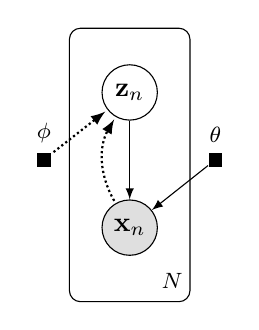
\begin{tikzpicture}

  % Nodes
  \node[latent] (z) {$\mbz_n$};
  \node[obs, below=of z] (x) {$\mbx_n$};

  \factor[empty, below=of z] {h} {} {} {};
  \factor[right=of h, xshift=0.5cm] {theta} {$\theta$} {} {};
  \factor[left=of h, xshift=-0.5cm] {phi} {$\phi$} {} {};

  % Edges
  \edge{z}{x};
  \draw[style=arrow, densely dotted, bend left] (x) to (z);
  \edge{theta}{x};
  \draw[style=arrow, densely dotted] (phi) to (z);

  % Plates
  \plate[inner sep=0.4cm, yshift=0.05cm,
    label={[xshift=-14pt,yshift=14pt]south east:$N$}] {plate1} {
    (z)(x)
  } {};

\end{tikzpicture}

  \label{sub:vae_math}
\end{subfigure}%
\begin{subfigure}{0.65\columnwidth}
  \centering
\begin{lstlisting}[language=python]
# Probabilistic model
z = Normal(mu=tf.zeros([N, d]), sigma=tf.ones([N, d]))
h = slim.fully_connected(z, 256)
x = Bernoulli(logits=slim.fully_connected(h, 28 * 28, activation_fn=None))

# Variational model
qx = tf.placeholder(tf.float32, [N, 28 * 28])
qh = slim.fully_connected(qx, 256)
qz = Normal(mu=slim.fully_connected(qh, d, activation_fn=None),
            sigma=slim.fully_connected(qh, d, activation_fn=tf.nn.softplus))
\end{lstlisting}
  \label{sub:vae_code}
\end{subfigure}
\caption{\Acrlong{VAE} for a data set of $28\times 28$ pixel images:
(left) graphical model, with dotted lines for the inference
model; (right) probabilistic program,
with 2-layer neural networks.
}
\label{fig:vae}
\end{figure}

\Cref{fig:vae}
implements
a \gls{VAE} \citep{kingma2014autoencoding,rezende2014stochastic} in Edward.
There are $N$ data points $\{x_n\}$ and $d$ latent
variables per data point $\{z_n\}$.
The program uses TensorFlow Slim \citep{guadarrama2016tensorflow}
to define the neural networks.
The probabilistic model is parameterized by a 2-layer neural network,
with 256 hidden units (and ReLU activation), and generates $28\times 28$
pixel images.  The variational model is parameterized by
a 2-layer inference network, with 256 hidden units and outputs
parameters of a normal posterior approximation.

The probabilistic program is concise.  Importantly, core elements of
the \gls{VAE}---such as its distributional assumptions and neural net
architectures---are all extensible.
Model compositionality enables it to be embedded into more complicated
models \citep{gregor2015draw,rezende2016one} and for other learning
tasks \citep{kingma2014semi}.
Inference compositionality (which we discuss later) enables it to be embedded into more
complicated algorithms, such as with expressive variational
approximations \citep{rezende2015variational,tran2016variational,kingma2016improving}
and alternative objectives \citep{ranganath2016operator,li2016variational,dieng2016chi}.


\subsection{Stochastic Control Flow and Model Parallelism}

\begin{figure}[!htb]
  \centering
  \input{img/dynamic_graph}
\caption{Computational graph for a probabilistic program with stochastic control flow.
}
\label{fig:dynamic}
\end{figure}

Random variables can also be integrated with control flow,
enabling probabilistic programs with stochastic control flow.
%
Stochastic control flow defines dynamic conditional dependencies,
known in the literature as contingent or existential dependencies
\citep{mansinghka2014venture,wu2016swift}.
See \Cref{fig:dynamic}, where $\mbx$ may or may not depend on $\mba$
for a given execution.

We use stochastic control flow to implement a Dirichlet process mixture model
in \Cref{appendix:dirichlet_process}.
Stochastic control flow produces difficulties for algorithms that leverage the
graph structure; the relationship of conditional dependencies
changes across execution traces.
Importantly, the computational graph provides
an elegant way of teasing out static conditional dependence structure
($\mbp$) from dynamic dependence structure ($\mba)$.  We can perform
model parallelism over the static structure with \glspl{GPU} and batch
training, and use generic computations to handle the dynamic
structure.

\input{model_compositionality}
\input{model_development}
\section{Compositional Representations for Inference}
\label{sec:inference}

We described random variables as a representation for building
rich probabilistic programs over computational graphs.  We now
describe a compositional representation for inference.
We desire two criteria: (a) support for many classes of
inference, where the form of the inferred posterior depends on the
algorithm; and (b) invariance of inference under the computational
graph, that is, the posterior can be further composed as part of
another model.

To explain our approach, we will use a simple hierarchical model as a
running example. \Cref{fig:hierarchical_model_example} displays a
joint distribution $p(\mbx, \mbz, \beta)$ of data $\mbx$, local
variables $\mbz$, and global variables $\beta$. The ideas here extend
to more expressive programs.

\begin{figure}[!h]
\begin{subfigure}{0.35\columnwidth}
  \centering
  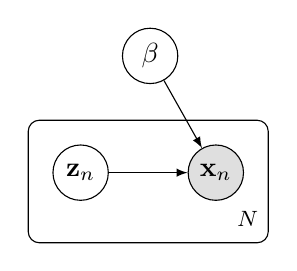
\begin{tikzpicture}

  % Nodes
  \node[latent]               (beta)      {$\beta$} ;
  \node[left=0.4cm of beta]               (betaph)      {} ;
  \node[latent, below=1.0cm of betaph] (z)    {$\mbz_n$} ;
  \node[obs, right=1.0cm of z]      (x)        {$\mbx_n$} ;

  % Edges
  % \edge{beta}{z};
  \edge{beta}{x};
  \edge{z}{x};

  % Plates
  \plate[inner sep=0.3cm,
    label={[xshift=-15pt,yshift=15pt]south east:$N$}] {plate1} {
    (x)(z)
  } {};

\end{tikzpicture}

\end{subfigure}%
\begin{subfigure}{0.6\columnwidth}
  \centering
\begin{lstlisting}[language=python]
N = 10000  # number of data points
D = 2  # data dimension
K = 5  # number of clusters

beta = Normal(mu=tf.zeros([K, D]), sigma=tf.ones([K, D]))
z = Categorical(logits=tf.zeros([N, K]))
x = Normal(mu=tf.gather(beta, z), sigma=tf.ones([N, D]))
\end{lstlisting}
\end{subfigure}
\caption{Hierarchical model: \textbf{(left)} graphical model; \textbf{(right)}
  probabilistic program. It is a mixture of Gaussians over
  $D$-dimensional data $\{x_n\}\in\mathbb{R}^{N\times D}$. There are
  $K$ latent cluster means $\beta\in\mathbb{R}^{K\times D}$.}
\label{fig:hierarchical_model_example}
\end{figure}

\subsection{Inference as Stochastic Graph Optimization}
\label{sub:inference}

The goal of inference is to
calculate the posterior distribution
$p(\mathbf{z}, \beta\mid \mathbf{x}_{\text{train}}; \mbtheta)$
given data $\mbx_{\text{train}}$,
where
$\mbtheta$ are any model parameters that we will compute point estimates
for.\footnote{%
For example, we could replace \texttt{x}'s \texttt{sigma}
argument with \texttt{tf.exp(tf.Variable(0.0))*tf.ones([N, D])}. This
defines a model parameter initialized at 0 and positive-constrained.}
We formalize this as the following optimization problem:
\begin{align}
  \label{eq:inference-optimization}
\min_{\mblambda,\mbtheta}
\mathcal{L}(
p(\mathbf{z}, \beta\mid \mathbf{x}_{\text{train}}; \mbtheta),~
q(\mathbf{z}, \beta; \mblambda)
),
\end{align}
where $q(\mathbf{z}, \beta; \mblambda)$ is an approximation to the
posterior $p(\mathbf{z}, \beta\g \mbx_{\text{train}};\mbtheta)$, and
$\mathcal{L}$ is a loss function with respect to $p$ and $q$.

The choice of approximation $q$, loss $\mathcal{L}$, and rules to update
parameters $\{\mbtheta,\mblambda\}$ are specified by an inference algorithm.
(Note $q$ can be nonparametric, such as a point or a collection of
samples.)

In Edward, we write this problem as follows:

\begin{lstlisting}[language=python]
inference = ed.Inference({beta: qbeta, z: qz}, data={x: x_train})
\end{lstlisting}

\texttt{Inference} is an abstract class which takes two inputs.  The
first is a collection of latent random variables \texttt{beta} and
\texttt{z}, associated to their ``posterior variables'' \texttt{qbeta} and
\texttt{qz} respectively. The second is a collection of observed random variables
\texttt{x}, which is associated to their realizations \texttt{x_train}.

The idea is that \texttt{Inference} defines and
solves the optimization in \Cref{eq:inference-optimization}. It
adjusts parameters of the distribution of \texttt{qbeta}
and \texttt{qz} (and any model parameters) to be close to the
posterior.

Class methods are available to finely control the inference. Calling
\texttt{inference.initialize()} builds a computational graph to update
$\{\mbtheta,\mblambda\}$. Calling \texttt{inference.update()} runs
this computation once to update $\{\mbtheta,\mblambda\}$; we call the
method in a loop until convergence. Importantly, no efficiency is lost
in Edward's language: the computational graph is the same as if it
were handwritten for a
specific model. This means the runtime is the same; also see our
experiments in \Cref{sub:gpu}.

A key concept in Edward is that there is no distinct ``model''
or ``inference'' block. A model is simply a collection of random
variables, and inference is a way of modifying parameters in that
collection subject to another. This reductionism offers
significant flexibility. For example, we can
infer only parts of a model (e.g.,
layer-wise training \citep{hinton2006fast}),
infer parts used in multiple models
(e.g., multi-task learning), or
plug in a posterior into a new model
(e.g., Bayesian updating).

\subsection{Classes of Inference}

The design of \texttt{Inference} is very general.  We describe
subclasses to represent many algorithms below: variational inference,
Monte Carlo, and \acrlongpl{GAN}.

Variational inference posits a family of approximating distributions
and finds the closest member in the family to the posterior
\citep{jordan1999introduction}.  In Edward, we build the variational
family in the graph; see \Cref{fig:inference} (left). For our running
example, the
family has mutable variables as parameters
$\mblambda=\{\pi,\mu,\sigma\}$, where
$q(\beta;\mu,\sigma) = \operatorname{Normal}(\beta; \mu,\sigma)$ and
$q(\mbz;\pi) = \operatorname{Categorical}(\mbz;\pi)$.

\begin{figure}[!h]
\begin{subfigure}{0.5\columnwidth}
  \centering
\begin{lstlisting}[language=Python]
qbeta = Normal(
  mu=tf.Variable(tf.zeros([K, D])),
  sigma=tf.exp(tf.Variable(tf.zeros([K, D]))))
qz = Categorical(
  logits=tf.Variable(tf.zeros([N, K])))

inference = ed.VariationalInference(
  {beta: qbeta, z: qz}, data={x: x_train})
\end{lstlisting}
\end{subfigure}%
\begin{subfigure}{0.5\columnwidth}
  \centering
\begin{lstlisting}[language=Python]
T = 10000  # number of samples
qbeta = Empirical(
  params=tf.Variable(tf.zeros([T, K, D])))
qz = Empirical(
  params=tf.Variable(tf.zeros([T, N])))

inference = ed.MonteCarlo(
  {beta: qbeta, z: qz}, data={x: x_train})
\end{lstlisting}
\end{subfigure}
\caption{\textbf{(left)} Variational inference. \textbf{(right)} Monte Carlo.}
\label{fig:inference}
\end{figure}

Specific variational algorithms inherit from the
\texttt{VariationalInference} class.  Each defines its own methods,
such as a loss function and gradient.
For example, we represent
\gls{MAP}
estimation with an approximating family (\texttt{qbeta} and
\texttt{qz}) of \texttt{PointMass} random variables, i.e., with all
probability mass concentrated at a point.
\texttt{MAP} inherits from \texttt{VariationalInference} and defines
the negative log joint density as the loss function; it uses existing optimizers inside
TensorFlow.
In \Cref{sub:recent}, we experiment with multiple gradient estimators
for black box variational inference \citep{ranganath:2014}. Each
estimator implements the same loss (an objective proportional to
the divergence $\operatorname{KL}(q\gg p)$) and a different update rule
(stochastic gradient).

Monte Carlo approximates the posterior using samples
\citep{robert1999monte}. Monte Carlo is an inference where the
approximating family is an empirical distribution,
$q(\beta; \{\beta^{(t)}\}) = \frac{1}{T}\sum_{t=1}^T \delta(\beta,
\beta^{(t)})$ and
$q(\mbz; \{\mbz^{(t)}\}) = \frac{1}{T}\sum_{t=1}^T \delta(\mbz,
\mbz^{(t)})$. The parameters are
$\mblambda=\{\beta^{(t)},\mbz^{(t)}\}$.  See \Cref{fig:inference}
(right).
Monte Carlo algorithms proceed by updating one sample
$\beta^{(t)},\mbz^{(t)}$ at a time in the empirical approximation.
Specific \glsunset{MC}\gls{MC} samplers determine the update rules:
they can use gradients such as in Hamiltonian Monte Carlo
\citep{neal2011mcmc} and graph
structure such as in sequential Monte Carlo \citep{doucet2001introduction}.



\begin{figure}[tb]
\begin{subfigure}{0.4\columnwidth}
  \centering
  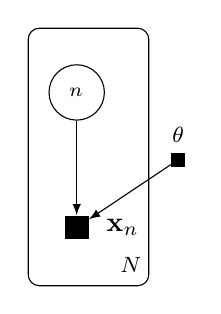
\begin{tikzpicture}

  % Nodes
  \node[latent] (eps0) {$\mbepsilon_n$};
  \factor[minimum size=0.3cm, below=1.2cm of eps0] {x} {} {} {};

  \factor[empty, below=of eps0] {h} {} {} {};
  \factor[right=of h, xshift=0.7cm] {theta} {$\theta$} {} {};

  \node[right=of x, xshift=-0.9cm] (xlabel) {$\mbx_n$};

  % Edges
  \edge{eps0}{x};
  \edge{theta}{x};

  % Plates
  \plate[inner sep=0.4cm, yshift=0.05cm,xshift=0.15cm,
    label={[xshift=-14pt,yshift=14pt]south east:$N$}] {plate1} {
    (eps0)(x)
  } {};

\end{tikzpicture}

\end{subfigure}%
\begin{subfigure}{0.6\columnwidth}
  \centering
\begin{lstlisting}[language=python]
def generative_network(eps):
  h = Dense(256, activation='relu')(eps)
  return Dense(28 * 28, activation=None)(h)

def discriminative_network(x):
  h = Dense(28 * 28, activation='relu')(x)
  return Dense(h, activation=None)(1)

# Probabilistic model
eps = Normal(mu=tf.zeros([N, d]), sigma=tf.ones([N, d]))
x = generative_network(eps)

inference = ed.GANInference(data={x: x_train},
    discriminator=discriminative_network)
\end{lstlisting}
\end{subfigure}
\caption{\Acrlongpl{GAN}:
\textbf{(left)} graphical model; \textbf{(right)} probabilistic program.
The model (generator) uses a parameterized function (discriminator)
for training.
}
\label{fig:gan}
\end{figure}

Edward also supports non-Bayesian methods such as \glspl{GAN}
\citep{goodfellow2014generative}.
See \Cref{fig:gan}.
The model posits
random noise \texttt{eps} over $N$ data points, each with $d$
dimensions; this random noise feeds into a
\texttt{generative_network} function, a neural network that outputs
real-valued data \texttt{x}.
In addition, there is a \texttt{discriminative_network}
which takes data as input and outputs the probability that
the data is real (in logit parameterization). We build
\texttt{GANInference}; running it optimizes parameters inside the two
neural network functions. This approach extends to many advances in
\glspl{GAN} (e.g., \citet{denton2015deep,li2015generative}).

Finally, one can design algorithms that would otherwise require tedious
algebraic manipulation. With symbolic algebra on nodes of the
computational graph, we can uncover conjugacy relationships between
random variables. Users can then integrate out variables to
automatically derive classical Gibbs \citep{gelfand1990sampling},
mean-field updates \citep{bishop2006pattern}, and exact inference.
These algorithms are being currently developed in Edward.

\subsection{Composing Inferences}

Core to Edward's design is that inference can be written as a collection
of separate inference programs. Below we demonstrate variational EM,
with an (approximate) E-step over local variables and an M-step over
global variables. We instantiate two algorithms, each of which
conditions on inferences from the other, and
we alternate with one update of each \citep{neal1993new},
\begin{lstlisting}[language=Python]
qbeta = PointMass(params=tf.Variable(tf.zeros([K, D])))
qz = Categorical(logits=tf.Variable(tf.zeros([N, K])))

inference_e = ed.VariationalInference({z: qz}, data={x: x_train, beta: qbeta})
inference_m = ed.MAP({beta: qbeta}, data={x: x_train, z: qz})
...
for _ in range(10000):
  inference_e.update()
  inference_m.update()
\end{lstlisting}
This extends to many other cases such as
exact EM for exponential families,
contrastive divergence \citep{hinton2002training},
pseudo-marginal methods \citep{andrieu2009pseudo},
and Gibbs sampling within variational inference
\citep{wang2012truncation,Hoffman:2015}.
We can also write message passing algorithms, which solve a collection
of local inference problems \citep{koller2009probabilistic}.  For
example, classical message passing uses exact local inference and
expectation propagation locally minimizes the Kullback-Leibler
divergence, $\text{KL}(p\gg q)$
\citep{minka2001expectation}.

\subsection{Data Subsampling}
\label{sub:batch_training}

Stochastic optimization \citep{bottou2010large} scales inference to
massive data and is key to
algorithms such as stochastic gradient Langevin dynamics
\citep{welling2011bayesian} and stochastic variational inference
\citep{hoffman2013stochastic}.  The idea is to cheaply estimate the
model's log joint density in an unbiased way.  At each step, one
subsamples a data set $\{x_m\}$ of size $M$ and then scales densities
with respect to local variables,
\begin{align*}
  \log p(\mbx, \mbz, \beta)
  & = \log p(\beta) +
  \sum_{n=1}^N\Big[\log p(x_n \g z_n, \beta) + \log p(z_n \g \beta)\Big]
  \\
  & \approx \log p(\beta) +
  \frac{N}{M}\sum_{m=1}^M\Big[\log p(x_m \g z_m, \beta) + \log p(z_m \g \beta)\Big].
\end{align*}
To support stochastic optimization, we represent only a subgraph of
the full model. This prevents reifying the full model, which can lead
to unreasonable memory consumption \citep{tristan2014augur}.  During
initialization, we pass in a dictionary to properly scale the
arguments. See \Cref{fig:hierachical_model_batch}.

\begin{figure}[!htb]
\begin{subfigure}{0.3\columnwidth}
  \centering
  \input{img/hierarchical_model}
  \label{sub:hierachical_model_math}
\end{subfigure}%
\begin{subfigure}{0.6\columnwidth}
  \centering
\begin{lstlisting}[language=python]
beta = Normal(mu=tf.zeros([K, D]), sigma=tf.ones([K, D]))
z = Categorical(logits=tf.zeros([M, K]))
x = Normal(mu=tf.gather(beta, z), sigma=tf.ones([M, D]))

qbeta = Normal(mu=tf.Variable(tf.zeros([K, D])),
               sigma=tf.nn.softplus(tf.Variable(tf.zeros([K, D]))))
qz = Categorical(logits=tf.Variable(tf.zeros([M, D])))

inference = ed.VariationalInference({beta: qbeta, z: qz}, data={x: x_batch})
inference.initialize(scale={x: float(N)/M, z: float(N)/M})
\end{lstlisting}
  \label{sub:hierarchical_model_code}
\end{subfigure}
\caption{Data subsampling with a hierarchical model. We define a
subgraph of the full model, forming a plate of size $M$
rather than $N$. We then scale all local random variables by $N/M$.}
\label{fig:hierachical_model_batch}
\end{figure}

Conceptually, the scale argument represents scaling for each random
variable's plate, as if we had seen that random variable $N / M$ as
many times.  As an example, \Cref{appendix:svi} shows how to implement
stochastic variational inference in Edward.
The approach extends naturally to streaming data
\citep{doucet2000on,broderick2013streaming,mcinerney2015population},
dynamic batch sizes, and data structures in which working on a
subgraph does not immediately apply
\citep{binder1997space,johnson2014stochastic,foti2014stochastic}.


\input{inference_classes}
\input{inference_compositionality}
\input{inference_data_subsampling}
\input{inference_development}
\subsection{Criticism}

We can never validate whether a model is true. In practice, ``all
models are wrong'' \citep{box1976science}. However, we can try to
uncover where the model goes wrong. Model criticism helps justify the
model as an approximation or point to good directions for revising the
model.

Edward explores model criticism using
\begin{itemize}
  \item point-based evaluations, such as mean squared error or
  classification accuracy;
  \item posterior predictive checks, for making probabilistic
  assessments of the model fit using discrepancy functions.
\end{itemize}

We describe them in detail below.

\input{criticism_point_evaluation}
\input{criticism_ppc}
\clearpage
\section{End-to-end Examples}
\label{sec:examples}

\subsection{Bayesian Linear Regression}

In supervised learning, the task is to infer hidden structure from
labeled data, comprised of training examples $\{(x_n, y_n)\}$.
Regression (typically) means the output $y$ takes continuous values.

\subsubsection{Data}

Simulate training and test sets of $500$ data points. They comprise
pairs of inputs $\mathbf{x}_n\in\mathbb{R}^{5}$ and outputs
$y_n\in\mathbb{R}$. They have a linear dependence of
\begin{align*}
  \mathbf{w}_{\text{true}}
  &=
  (-1.25, 4.51, 2.32, 0.99, -3.44).
\end{align*}
with normally distributed noise.

\begin{lstlisting}
def build_toy_dataset(N, w, noise_std=0.1):
  D = len(w)
  x = np.random.randn(N, D).astype(np.float32)
  y = np.dot(x, w) + np.random.normal(0, noise_std, size=N)
  return x, y

N = 500  # number of  data points
D = 5  # number of  features

w_true = 10 * (np.random.rand(D) - 0.5)
X_train, y_train = build_toy_dataset(N, w_true)
X_test, y_test = build_toy_dataset(N, w_true)
\end{lstlisting}

\subsubsection{Model}

Posit the model as Bayesian linear regression. It relates
outputs $y\in\mathbb{R}$, also known as the response, given
a vector of inputs
$\mathbf{x}\in\mathbb{R}^D$, also known as the features or covariates.
The model assumes a
linear relationship between these two random variables
\citep{murphy2012machine}.

For a set of $N$ data points $(\mathbf{X},\mathbf{y})=\{(\mathbf{x}_n, y_n)\}$,
the model posits the following conditional relationships:
\begin{align*}
  p(\mathbf{w})
  &=
  \text{Normal}(\mathbf{w} \mid \mathbf{0}, \sigma_w^2\mathbf{I}),
  \\[1.5ex]
  p(b)
  &=
  \text{Normal}(b \mid 0, \sigma_b^2),
  \\
  p(\mathbf{y} \mid \mathbf{w}, b, \mathbf{X})
  &=
  \prod_{n=1}^N
  \text{Normal}(y_n \mid \mathbf{x}_n^\top\mathbf{w} + b, \sigma_y^2).
\end{align*}
The latent variables are the linear model's weights $\mathbf{w}$ and
intercept $b$, also known as the bias.
Assume $\sigma_w^2,\sigma_b^2$ are known prior variances and $\sigma_y^2$ is a
known likelihood variance. The mean of the likelihood is given by a
linear transformation of the inputs $\mathbf{x}_n$.

\begin{lstlisting}
X = tf.placeholder(tf.float32, [N, D])
w = Normal(mu=tf.zeros(D), sigma=tf.ones(D))
b = Normal(mu=tf.zeros(1), sigma=tf.ones(1))
y = Normal(mu=ed.dot(X, w) + b, sigma=tf.ones(N))
\end{lstlisting}

\subsubsection{Inference}

We now turn to inferring the posterior using variational inference.
Define the variational model to be a fully factorized normal across
the weights.
\begin{lstlisting}
qw = Normal(mu=tf.Variable(tf.random_normal([D])),
            sigma=tf.nn.softplus(tf.Variable(tf.random_normal([D]))))
qb = Normal(mu=tf.Variable(tf.random_normal([1])),
            sigma=tf.nn.softplus(tf.Variable(tf.random_normal([1]))))
\end{lstlisting}

Run variational inference with the Kullback-Leibler divergence, using a
default of $1000$ iterations.
\begin{lstlisting}
inference = ed.KLqp({w: qw, b: qb}, data={X: X_train, y: y_train})
inference.run()
\end{lstlisting}
In this case \texttt{KLqp} defaults to minimizing the
$\text{KL}(q\|p)$ divergence measure using the reparameterization
gradient.
Minimizing this divergence metric is equivalent to maximizing the
evidence lower bound (\textsc{elbo}). Figure\nobreakspace \ref{fig:supervised-elbo} shows the
progression of the \textsc{elbo} across iterations; variational inference
appears to converge in approximately 200 iterations.

\begin{figure}[htb]
\centering
% This file was created by matplotlib2tikz v0.5.15.
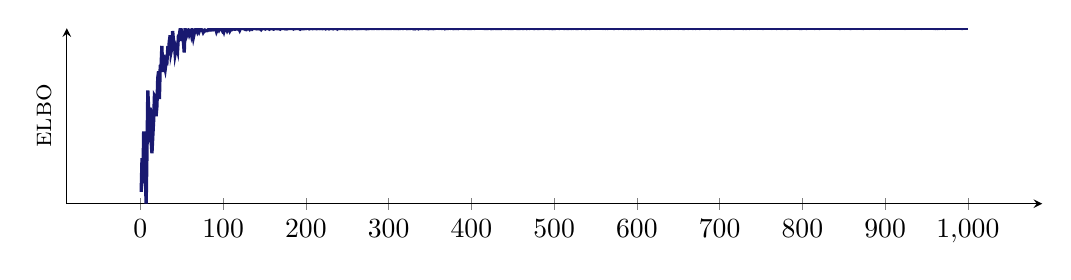
\begin{tikzpicture}

\begin{axis}[
width=5.5in,
height=1.5in,
axis lines=left,
enlarge x limits=0.09,
ylabel={\textsc{elbo}},
ylabel near ticks,
ytick=\empty,
% legend entries={{$\textsc{elbo}$}},
% legend style={draw=none, at={(1.0,1.0)}, anchor=north east,font=\small},
% legend cell align=left,
]
\addplot [very thick, MidnightBlue]
table {%
1 -24832.922
2 -19803.498
3 -23561.203
4 -15824.293
5 -20963.410
6 -22910.539
7 -26589.451
8 -18808.270
9 -9747.762
10 -12387.727
11 -17470.422
12 -12321.565
13 -17315.900
14 -19084.033
15 -16630.318
16 -14351.264
17 -10512.238
18 -10711.228
19 -13574.313
20 -12119.984
21 -7890.950
22 -6892.946
23 -11034.027
24 -6176.863
25 -6172.959
26 -3107.659
27 -7020.251
28 -4452.798
29 -6089.138
30 -6615.671
31 -5675.927
32 -5712.329
33 -3730.986
34 -3880.640
35 -2384.833
36 -1533.137
37 -4068.863
38 -3454.978
39 -919.619
40 -2226.556
41 -2632.443
42 -4297.725
43 -3595.808
44 -3212.551
45 -3748.414
46 -1623.859
47 -1570.649
48 -740.249
49 -2372.888
50 -1205.361
51 -1917.089
52 -2547.169
53 -4118.985
54 -621.050
55 -757.427
56 -1556.877
57 -1209.368
58 -889.026
59 -1362.566
60 -966.671
61 -845.125
62 -1561.782
63 -1137.697
64 -1877.333
65 -1303.988
66 -1014.029
67 -591.169
68 -611.487
69 -991.204
70 -681.929
71 -984.964
72 -658.884
73 -763.687
74 -714.870
75 -763.138
76 -1100.189
77 -909.522
78 -784.309
79 -874.663
80 -824.489
81 -841.660
82 -717.680
83 -575.089
84 -705.678
85 -583.816
86 -738.280
87 -730.617
88 -509.557
89 -653.959
90 -559.539
91 -562.100
92 -984.054
93 -689.061
94 -538.112
95 -761.587
96 -533.470
97 -559.037
98 -589.960
99 -838.655
100 -584.534
101 -962.970
102 -518.553
103 -612.928
104 -522.122
105 -845.492
106 -619.405
107 -576.229
108 -865.849
109 -589.953
110 -508.640
111 -669.911
112 -607.241
113 -560.890
114 -629.296
115 -626.430
116 -568.982
117 -605.701
118 -629.469
119 -537.192
120 -781.661
121 -500.954
122 -540.029
123 -535.272
124 -529.918
125 -578.479
126 -601.557
127 -682.052
128 -701.809
129 -529.723
130 -532.800
131 -542.383
132 -670.603
133 -499.615
134 -529.973
135 -633.945
136 -542.460
137 -530.477
138 -531.029
139 -548.708
140 -503.343
141 -576.710
142 -550.642
143 -573.576
144 -599.329
145 -514.116
146 -676.929
147 -520.751
148 -549.704
149 -519.155
150 -532.308
151 -606.272
152 -529.381
153 -521.502
154 -515.503
155 -566.671
156 -627.266
157 -519.156
158 -505.319
159 -548.680
160 -574.648
161 -624.666
162 -565.911
163 -527.196
164 -516.848
165 -555.894
166 -555.441
167 -552.636
168 -533.432
169 -616.256
170 -514.473
171 -515.411
172 -521.036
173 -542.845
174 -538.216
175 -580.167
176 -550.768
177 -594.729
178 -550.794
179 -519.260
180 -524.028
181 -539.773
182 -536.005
183 -500.866
184 -503.364
185 -594.558
186 -507.863
187 -545.172
188 -514.240
189 -505.776
190 -533.364
191 -512.997
192 -563.213
193 -631.401
194 -531.153
195 -554.997
196 -543.574
197 -572.771
198 -549.754
199 -526.739
200 -545.172
201 -499.916
202 -499.685
203 -518.962
204 -577.682
205 -516.530
206 -507.992
207 -502.159
208 -558.325
209 -527.241
210 -501.722
211 -530.918
212 -531.191
213 -565.879
214 -506.361
215 -509.624
216 -507.127
217 -544.332
218 -507.483
219 -526.420
220 -562.512
221 -530.384
222 -518.334
223 -506.957
224 -583.284
225 -501.156
226 -521.283
227 -522.312
228 -580.823
229 -530.023
230 -522.596
231 -530.254
232 -501.868
233 -575.415
234 -521.655
235 -500.199
236 -534.586
237 -503.783
238 -601.045
239 -501.512
240 -530.466
241 -518.048
242 -510.544
243 -491.884
244 -524.739
245 -505.006
246 -534.611
247 -549.057
248 -499.555
249 -556.432
250 -526.919
251 -533.946
252 -506.801
253 -546.932
254 -512.135
255 -495.986
256 -556.187
257 -507.510
258 -511.102
259 -502.828
260 -513.216
261 -508.672
262 -558.700
263 -527.179
264 -543.484
265 -506.969
266 -532.850
267 -506.210
268 -516.335
269 -495.212
270 -517.379
271 -528.253
272 -497.483
273 -572.889
274 -546.855
275 -498.365
276 -543.458
277 -518.540
278 -493.510
279 -517.002
280 -536.921
281 -509.926
282 -525.150
283 -520.514
284 -500.861
285 -506.285
286 -520.448
287 -505.468
288 -514.473
289 -510.371
290 -501.895
291 -517.209
292 -518.540
293 -522.171
294 -527.152
295 -498.954
296 -497.152
297 -523.719
298 -496.689
299 -520.748
300 -518.319
301 -524.671
302 -510.265
303 -510.676
304 -508.489
305 -497.077
306 -526.555
307 -520.639
308 -517.420
309 -523.865
310 -537.216
311 -503.112
312 -544.220
313 -510.059
314 -521.773
315 -505.111
316 -503.992
317 -524.134
318 -512.138
319 -498.316
320 -504.593
321 -499.354
322 -546.580
323 -514.315
324 -515.279
325 -512.180
326 -517.124
327 -506.894
328 -494.740
329 -533.814
330 -569.474
331 -502.172
332 -571.643
333 -513.843
334 -510.310
335 -503.516
336 -575.851
337 -504.016
338 -534.706
339 -497.825
340 -512.104
341 -518.426
342 -503.748
343 -509.475
344 -499.075
345 -533.529
346 -504.493
347 -500.657
348 -567.336
349 -532.630
350 -514.995
351 -526.937
352 -513.165
353 -531.044
354 -550.746
355 -504.847
356 -521.411
357 -498.129
358 -508.284
359 -506.762
360 -506.213
361 -512.521
362 -499.582
363 -501.453
364 -519.875
365 -511.799
366 -495.873
367 -506.501
368 -565.908
369 -509.649
370 -515.521
371 -526.465
372 -518.555
373 -502.669
374 -504.838
375 -509.898
376 -504.504
377 -510.423
378 -542.953
379 -504.786
380 -526.260
381 -521.690
382 -531.245
383 -516.041
384 -540.712
385 -504.336
386 -504.113
387 -502.955
388 -501.416
389 -497.498
390 -514.521
391 -500.098
392 -515.770
393 -499.772
394 -508.010
395 -507.638
396 -520.820
397 -529.995
398 -510.079
399 -524.253
400 -514.175
401 -502.353
402 -508.909
403 -504.541
404 -512.921
405 -504.037
406 -499.760
407 -503.540
408 -506.858
409 -499.937
410 -498.388
411 -499.468
412 -498.646
413 -505.261
414 -508.928
415 -503.252
416 -519.530
417 -510.247
418 -510.240
419 -523.058
420 -519.503
421 -500.548
422 -506.653
423 -502.075
424 -546.387
425 -530.292
426 -540.231
427 -499.338
428 -506.619
429 -515.662
430 -529.709
431 -529.118
432 -508.514
433 -523.447
434 -517.518
435 -501.008
436 -537.748
437 -501.082
438 -504.598
439 -503.611
440 -500.672
441 -510.425
442 -499.719
443 -511.103
444 -505.230
445 -511.932
446 -500.884
447 -539.216
448 -529.175
449 -537.471
450 -524.694
451 -502.843
452 -496.148
453 -506.900
454 -507.648
455 -509.699
456 -520.198
457 -519.453
458 -506.753
459 -518.399
460 -495.285
461 -505.901
462 -522.508
463 -527.759
464 -508.374
465 -504.670
466 -503.456
467 -539.282
468 -496.581
469 -500.324
470 -515.431
471 -508.935
472 -501.346
473 -497.972
474 -500.478
475 -521.828
476 -542.320
477 -506.258
478 -495.614
479 -505.659
480 -514.763
481 -512.574
482 -516.924
483 -497.719
484 -512.537
485 -496.289
486 -503.220
487 -519.888
488 -510.391
489 -496.645
490 -501.112
491 -507.252
492 -503.251
493 -496.841
494 -518.408
495 -503.256
496 -510.145
497 -508.684
498 -541.055
499 -510.272
500 -508.380
501 -526.208
502 -505.449
503 -508.021
504 -501.584
505 -496.387
506 -517.301
507 -506.702
508 -501.748
509 -500.537
510 -496.489
511 -507.099
512 -513.221
513 -514.784
514 -494.533
515 -511.332
516 -506.822
517 -524.429
518 -496.344
519 -510.229
520 -501.417
521 -520.455
522 -499.426
523 -511.695
524 -504.585
525 -503.283
526 -511.264
527 -515.652
528 -509.630
529 -511.151
530 -506.625
531 -505.202
532 -497.890
533 -510.685
534 -506.627
535 -507.428
536 -504.274
537 -509.759
538 -522.179
539 -523.910
540 -504.896
541 -502.109
542 -506.130
543 -517.468
544 -500.137
545 -498.487
546 -501.097
547 -500.590
548 -507.752
549 -499.834
550 -502.212
551 -504.722
552 -500.224
553 -504.556
554 -504.306
555 -503.422
556 -502.557
557 -498.314
558 -505.328
559 -510.563
560 -504.654
561 -499.723
562 -516.698
563 -501.232
564 -508.030
565 -510.750
566 -500.261
567 -498.932
568 -502.426
569 -505.373
570 -498.250
571 -503.679
572 -514.284
573 -512.353
574 -499.591
575 -499.622
576 -502.963
577 -496.011
578 -511.305
579 -506.990
580 -500.962
581 -503.827
582 -501.354
583 -500.075
584 -515.265
585 -504.798
586 -513.242
587 -498.378
588 -497.362
589 -516.766
590 -510.508
591 -502.276
592 -523.989
593 -513.169
594 -499.786
595 -497.028
596 -508.840
597 -505.038
598 -516.705
599 -510.934
600 -516.177
601 -503.793
602 -500.364
603 -517.858
604 -502.610
605 -511.523
606 -510.420
607 -498.120
608 -511.895
609 -498.941
610 -497.207
611 -500.341
612 -507.238
613 -498.622
614 -499.937
615 -504.822
616 -513.693
617 -503.950
618 -503.808
619 -507.735
620 -510.914
621 -496.255
622 -499.346
623 -503.904
624 -519.045
625 -500.680
626 -506.674
627 -504.924
628 -523.276
629 -515.196
630 -503.100
631 -506.020
632 -497.345
633 -502.293
634 -517.487
635 -497.628
636 -506.710
637 -515.729
638 -500.366
639 -500.153
640 -512.040
641 -498.316
642 -502.173
643 -504.783
644 -501.223
645 -500.492
646 -509.528
647 -498.987
648 -502.461
649 -502.459
650 -511.940
651 -505.319
652 -502.409
653 -501.323
654 -507.214
655 -499.913
656 -530.570
657 -512.025
658 -508.064
659 -503.212
660 -499.930
661 -505.267
662 -514.629
663 -500.950
664 -505.419
665 -505.696
666 -497.856
667 -508.020
668 -510.515
669 -502.513
670 -503.230
671 -515.594
672 -496.592
673 -503.725
674 -500.498
675 -499.564
676 -516.964
677 -503.196
678 -505.050
679 -500.136
680 -499.966
681 -496.349
682 -506.102
683 -500.523
684 -500.489
685 -506.254
686 -500.197
687 -501.952
688 -519.274
689 -499.919
690 -503.175
691 -504.537
692 -499.757
693 -502.693
694 -498.425
695 -502.422
696 -504.033
697 -503.499
698 -517.570
699 -505.387
700 -500.494
701 -509.516
702 -507.658
703 -503.182
704 -506.818
705 -498.547
706 -496.710
707 -501.242
708 -499.315
709 -509.116
710 -497.264
711 -499.059
712 -498.797
713 -497.495
714 -508.322
715 -506.021
716 -505.151
717 -512.350
718 -509.821
719 -501.822
720 -500.342
721 -495.944
722 -501.319
723 -502.265
724 -501.476
725 -503.717
726 -504.835
727 -498.007
728 -511.145
729 -512.207
730 -495.707
731 -505.319
732 -517.518
733 -500.396
734 -498.152
735 -496.250
736 -511.999
737 -502.275
738 -500.993
739 -501.565
740 -502.559
741 -502.758
742 -499.287
743 -504.771
744 -497.680
745 -501.568
746 -508.972
747 -501.550
748 -499.927
749 -506.345
750 -505.651
751 -505.419
752 -510.120
753 -510.091
754 -503.827
755 -495.517
756 -504.425
757 -508.215
758 -503.453
759 -500.999
760 -499.582
761 -494.836
762 -494.701
763 -510.070
764 -506.157
765 -505.592
766 -503.926
767 -496.379
768 -505.495
769 -513.070
770 -501.799
771 -499.353
772 -503.395
773 -495.691
774 -512.763
775 -503.920
776 -509.860
777 -504.101
778 -501.568
779 -504.793
780 -507.061
781 -507.604
782 -526.716
783 -506.790
784 -498.373
785 -499.975
786 -507.128
787 -504.331
788 -498.521
789 -500.208
790 -502.291
791 -505.092
792 -501.648
793 -504.965
794 -499.602
795 -498.995
796 -506.491
797 -517.031
798 -502.801
799 -520.839
800 -505.293
801 -500.011
802 -500.577
803 -499.595
804 -501.668
805 -519.901
806 -501.038
807 -498.892
808 -500.228
809 -506.250
810 -499.398
811 -504.560
812 -497.615
813 -499.576
814 -501.447
815 -511.313
816 -496.942
817 -505.703
818 -499.415
819 -505.719
820 -508.774
821 -516.705
822 -498.311
823 -496.940
824 -503.315
825 -498.452
826 -503.590
827 -496.700
828 -505.269
829 -497.584
830 -497.001
831 -503.100
832 -500.741
833 -497.989
834 -500.802
835 -507.409
836 -498.523
837 -495.966
838 -501.295
839 -505.662
840 -504.811
841 -499.122
842 -508.961
843 -503.303
844 -504.203
845 -519.745
846 -510.439
847 -500.487
848 -501.894
849 -499.687
850 -501.675
851 -508.799
852 -498.292
853 -502.280
854 -501.178
855 -500.300
856 -500.580
857 -508.458
858 -508.773
859 -508.863
860 -500.323
861 -499.661
862 -507.355
863 -500.921
864 -503.958
865 -502.179
866 -508.534
867 -501.389
868 -503.068
869 -500.272
870 -501.099
871 -508.925
872 -495.506
873 -508.646
874 -509.754
875 -497.287
876 -500.348
877 -498.079
878 -507.489
879 -497.506
880 -502.639
881 -508.541
882 -506.465
883 -500.146
884 -498.308
885 -496.296
886 -501.985
887 -497.248
888 -503.042
889 -497.521
890 -498.882
891 -497.171
892 -499.977
893 -510.504
894 -500.521
895 -508.016
896 -507.364
897 -500.553
898 -503.865
899 -503.870
900 -508.329
901 -496.506
902 -503.336
903 -498.970
904 -504.545
905 -500.459
906 -499.504
907 -500.112
908 -499.521
909 -502.887
910 -498.618
911 -499.378
912 -497.413
913 -497.134
914 -501.098
915 -496.958
916 -501.820
917 -502.435
918 -504.083
919 -496.351
920 -496.450
921 -501.246
922 -498.509
923 -498.536
924 -514.812
925 -501.555
926 -500.779
927 -499.724
928 -499.486
929 -500.125
930 -503.387
931 -499.596
932 -498.748
933 -498.041
934 -506.005
935 -501.958
936 -504.011
937 -506.678
938 -502.875
939 -502.559
940 -503.202
941 -506.613
942 -501.716
943 -504.522
944 -508.776
945 -503.441
946 -495.678
947 -502.650
948 -496.957
949 -499.896
950 -502.784
951 -506.385
952 -504.492
953 -498.185
954 -498.434
955 -502.333
956 -498.237
957 -502.103
958 -500.029
959 -512.904
960 -500.114
961 -515.571
962 -497.049
963 -516.198
964 -500.885
965 -510.297
966 -505.765
967 -497.950
968 -500.930
969 -509.485
970 -503.810
971 -499.977
972 -495.887
973 -516.036
974 -499.370
975 -499.582
976 -499.370
977 -503.561
978 -505.015
979 -501.830
980 -498.268
981 -501.339
982 -497.624
983 -500.158
984 -496.479
985 -498.115
986 -496.805
987 -504.025
988 -498.504
989 -505.092
990 -503.705
991 -501.599
992 -506.653
993 -520.895
994 -503.029
995 -500.051
996 -499.964
997 -498.315
998 -500.947
999 -505.222
1000 -507.608
};
\end{axis}

\end{tikzpicture}

\caption{The evidence lower bound (\textsc{elbo}) as a function of iterations.
Variational inference maximizes this quantity iteratively; in this case, the
algorithm appears to have converged in approximately 200 iterations.}
\label{fig:supervised-elbo}
\end{figure}

Figure\nobreakspace \ref{fig:supervised-betas} shows the resulting posteriors from  variational
inference. We plot the marginal posteriors for each component of the vector of
coefficients $\beta$. The vertical lines indicate the ``true'' values of the
coefficients that we simulated above.

\begin{figure}[htb]
\centering
% This file was created by matplotlib2tikz v0.5.15.
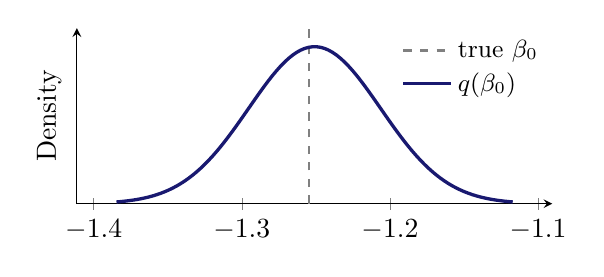
\begin{tikzpicture}

\begin{axis}[
width=3.0in,
height=1.5in,
axis lines=left,
enlarge x limits=0.1,
ylabel={Density},
ylabel near ticks,
ytick=\empty,
legend entries={{true $\beta_0$}, {$q(\beta_0)$}},
legend style={draw=none, at={(1.0,1.0)}, anchor=north east,font=\small},
legend cell align=left,
]
\addplot [thick, dashed, gray]
table {%
-1.25459881152638 0
-1.25459881152638 10
};
\addplot [very thick, MidnightBlue]
table {%
-1.3846001252532 0.0994103432712143
-1.38189822457957 0.119013603277019
-1.37919632390593 0.141960143663186
-1.3764944232323 0.168710087816997
-1.37379252255866 0.199765491467325
-1.37109062188503 0.23567020520197
-1.36838872121139 0.277008877312448
-1.36568682053776 0.324404962879766
-1.36298491986412 0.378517608358809
-1.36028301919048 0.440037289017542
-1.35758111851685 0.509680089993057
-1.35487921784321 0.588180540878532
-1.35217731716958 0.676282938940386
-1.34947541649594 0.774731127379731
-1.34677351582231 0.884256732367532
-1.34407161514867 1.00556590551315
-1.34136971447504 1.1393246663063
-1.3386678138014 1.28614299094489
-1.33596591312777 1.44655784857285
-1.33326401245413 1.62101544176614
-1.3305621117805 1.80985296332854
-1.32786021110686 2.01328023408348
-1.32515831043323 2.23136163420829
-1.32245640975959 2.46399878150339
-1.31975450908596 2.71091444157125
-1.31705260841232 2.97163817504537
-1.31435070773869 3.245494233803
-1.31164880706505 3.53159220986514
-1.30894690639142 3.82882091618547
-1.30624500571778 4.13584593700778
-1.30354310504415 4.45111122675914
-1.30084120437051 4.77284506101201
-1.29813930369688 5.0990705520425
-1.29543740302324 5.42762083676813
-1.29273550234961 5.75615892887182
-1.29003360167597 6.08220210282844
-1.28733170100234 6.40315054899689
-1.2846298003287 6.71631990999255
-1.28192789965507 7.01897718355629
-1.27922599898143 7.30837936054445
-1.2765240983078 7.58181406287413
-1.27382219763416 7.83664135941491
-1.27112029696053 8.07033587163715
-1.26841839628689 8.28052823841812
-1.26571649561326 8.46504499312375
-1.26301459493962 8.62194591739624
-1.26031269426599 8.74955797547933
-1.25761079359235 8.84650499987558
-1.25490889291872 8.91173239208829
-1.25220699224508 8.94452621859864
-1.24950509157145 8.94452621859864
-1.24680319089781 8.91173239208829
-1.24410129022418 8.84650499987558
-1.24139938955054 8.74955797547933
-1.23869748887691 8.62194591739624
-1.23599558820327 8.46504499312375
-1.23329368752964 8.28052823841812
-1.230591786856 8.07033587163715
-1.22788988618237 7.83664135941491
-1.22518798550873 7.58181406287413
-1.2224860848351 7.30837936054445
-1.21978418416146 7.01897718355629
-1.21708228348783 6.71631990999255
-1.21438038281419 6.40315054899689
-1.21167848214056 6.08220210282844
-1.20897658146692 5.75615892887182
-1.20627468079329 5.42762083676813
-1.20357278011965 5.0990705520425
-1.20087087944602 4.77284506101201
-1.19816897877238 4.45111122675914
-1.19546707809875 4.13584593700778
-1.19276517742511 3.82882091618547
-1.19006327675147 3.53159220986514
-1.18736137607784 3.245494233803
-1.1846594754042 2.97163817504537
-1.18195757473057 2.71091444157125
-1.17925567405693 2.46399878150339
-1.1765537733833 2.23136163420829
-1.17385187270966 2.01328023408348
-1.17114997203603 1.80985296332852
-1.16844807136239 1.62101544176614
-1.16574617068876 1.44655784857284
-1.16304427001512 1.28614299094489
-1.16034236934149 1.1393246663063
-1.15764046866785 1.00556590551315
-1.15493856799422 0.884256732367532
-1.15223666732058 0.774731127379731
-1.14953476664695 0.676282938940386
-1.14683286597331 0.588180540878532
-1.14413096529968 0.509680089993057
-1.14142906462604 0.440037289017542
-1.13872716395241 0.378517608358809
-1.13602526327877 0.324404962879766
-1.13332336260514 0.277008877312448
-1.1306214619315 0.23567020520197
-1.12791956125787 0.199765491467325
-1.12521766058423 0.168710087816997
-1.1225157599106 0.141960143663186
-1.11981385923696 0.119013603277019
-1.11711195856333 0.0994103432712143
};
\end{axis}

\end{tikzpicture}

% This file was created by matplotlib2tikz v0.5.15.
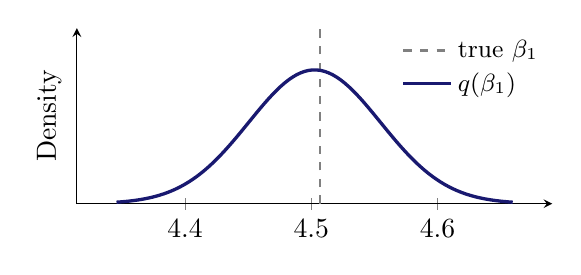
\begin{tikzpicture}

\begin{axis}[
width=3.0in,
height=1.5in,
axis lines=left,
enlarge x limits=0.1,
ylabel={Density},
ylabel near ticks,
ytick=\empty,
legend entries={{true $\beta_1$}, {$q(\beta_1)$}},
legend style={draw=none, at={(1.0,1.0)}, anchor=north east,font=\small},
legend cell align=left,
]
\addplot [thick, dashed, gray]
table {%
4.50714306409916 0
4.50714306409916 10
};
\addplot [very thick, MidnightBlue]
table {%
4.34573828801513 0.0847196368493868
4.34890870851549 0.10142595748068
4.35207912901586 0.120981493700508
4.35524954951622 0.143778372575268
4.35841997001659 0.170244456816511
4.36159039051695 0.200843227615254
4.36476081101732 0.236072934844829
4.36793123151768 0.276464900360839
4.37110165201805 0.32258086297689
4.37427207251841 0.375009260596227
4.37744249301878 0.434360356404465
4.38061291351914 0.501260132350176
4.38378333401951 0.576342894603564
4.38695375451987 0.660242562370592
4.39012417502024 0.753582643240854
4.3932945955206 0.856964934833564
4.39646501602097 0.970957033310708
4.39963543652134 1.0960787735333
4.4028058570217 1.23278777217752
4.40597627752207 1.3814642926944
4.40914669802243 1.5423956980579
4.4123171185228 1.71576080209543
4.41548753902316 1.9016144709815
4.41865795952353 2.09987286128549
4.42182838002389 2.31029970787936
4.42499880052426 2.5324940921969
4.42816922102462 2.7658801271254
4.43133964152499 3.00969898779668
4.43451006202535 3.26300369666362
4.43768048252572 3.52465703586171
4.44085090302608 3.79333290982064
4.44402132352645 4.06752141680225
4.44719174402681 4.34553781048589
4.45036216452718 4.62553544345631
4.45353258502754 4.90552268561157
4.45670300552791 5.18338370475588
4.45987342602827 5.45690288708667
4.46304384652864 5.72379256539229
4.466214267029 5.98172361625076
4.46938468752937 6.22835838815748
4.47255510802973 6.46138533405777
4.4757255285301 6.67855464775127
4.47889594903046 6.8777141472326
4.48206636953083 7.05684461189273
4.48523679003119 7.21409376662747
4.48840721053156 7.34780811554017
4.49157763103192 7.45656186150507
4.49474805153229 7.53918220492418
4.49791847203266 7.59477039423177
4.50108889253302 7.62271799989771
4.50425931303339 7.62271799989771
4.50742973353375 7.59477039423177
4.51060015403412 7.53918220492418
4.51377057453448 7.45656186150507
4.51694099503485 7.34780811554017
4.52011141553521 7.21409376662747
4.52328183603558 7.05684461189273
4.52645225653594 6.8777141472326
4.52962267703631 6.67855464775127
4.53279309753667 6.46138533405777
4.53596351803704 6.22835838815748
4.5391339385374 5.98172361625076
4.54230435903777 5.72379256539229
4.54547477953813 5.45690288708667
4.5486452000385 5.18338370475588
4.55181562053886 4.90552268561157
4.55498604103923 4.62553544345631
4.55815646153959 4.34553781048589
4.56132688203996 4.06752141680225
4.56449730254032 3.79333290982064
4.56766772304069 3.52465703586171
4.57083814354105 3.26300369666362
4.57400856404142 3.00969898779668
4.57717898454178 2.7658801271254
4.58034940504215 2.5324940921969
4.58351982554252 2.31029970787936
4.58669024604288 2.09987286128549
4.58986066654325 1.9016144709815
4.59303108704361 1.71576080209543
4.59620150754398 1.5423956980579
4.59937192804434 1.3814642926944
4.60254234854471 1.23278777217752
4.60571276904507 1.0960787735333
4.60888318954544 0.970957033310708
4.6120536100458 0.856964934833564
4.61522403054617 0.753582643240854
4.61839445104653 0.660242562370592
4.6215648715469 0.576342894603564
4.62473529204726 0.501260132350176
4.62790571254763 0.434360356404465
4.63107613304799 0.375009260596227
4.63424655354836 0.32258086297689
4.63741697404872 0.276464900360839
4.64058739454909 0.236072934844829
4.64375781504945 0.200843227615254
4.64692823554982 0.170244456816511
4.65009865605018 0.143778372575268
4.65326907655055 0.120981493700508
4.65643949705091 0.10142595748068
4.65960991755128 0.0847196368493868
};
\end{axis}

\end{tikzpicture}


\medskip

% This file was created by matplotlib2tikz v0.5.15.
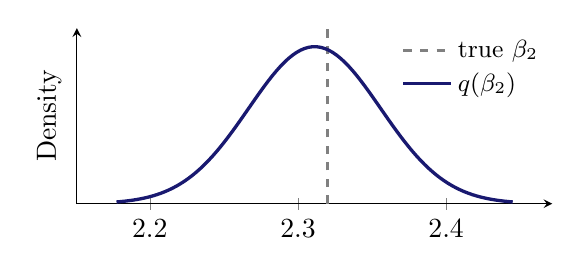
\begin{tikzpicture}

\begin{axis}[
width=3.0in,
height=1.5in,
axis lines=left,
enlarge x limits=0.1,
ylabel={Density},
ylabel near ticks,
ytick=\empty,
legend entries={{true $\beta_2$}, {$q(\beta_2)$}},
legend style={draw=none, at={(1.0,1.0)}, anchor=north east,font=\small},
legend cell align=left,
]
\addplot [thick, dashed, gray]
table {%
2.31993941811405 0
2.31993941811405 10
};
\addplot [very thick, MidnightBlue]
table {%
2.17749552056193 0.0994200051212747
2.18019715865905 0.119025170399235
2.18289879675616 0.141973940996314
2.18560043485327 0.168726485019929
2.18830207295039 0.199784906994549
2.1910037110475 0.235693110365672
2.19370534914461 0.277035800247729
2.19640698724172 0.324436492316309
2.19910862533884 0.378554397089809
2.20181026343595 0.440080056944581
2.20451190153306 0.509729626615162
2.20721353963017 0.588237707084861
2.20991517772729 0.676348667959524
2.2126168158244 0.774806424735553
2.21531845392151 0.884342674691867
2.21802009201863 1.00566363806981
2.22072173011574 1.13943539909057
2.22342336821285 1.28626799323666
2.22612500630996 1.44669844184086
2.22882664440708 1.62117299084632
2.23152828250419 1.8100288658291
2.2342299206013 2.01347590800542
2.23693155869842 2.23157850380988
2.23963319679553 2.46423826148096
2.24233483489264 2.71117791967622
2.24503647298975 2.97192699330649
2.24773811108687 3.24580966857194
2.25043974918398 3.53193545095336
2.25314138728109 3.82919304540647
2.25584302537821 4.13624790648096
2.25854466347532 4.45154383736945
2.26124630157243 4.77330894144763
2.26394793966954 5.09956613885468
2.26664957776666 5.42814835590733
2.26935121586377 5.75671837915301
2.27205285396088 6.0827932417665
2.274754492058 6.40377288142713
2.27745613015511 6.71697267985326
2.28015776825222 7.01965936916085
2.28285940634933 7.3090896736089
2.28556104444645 7.58255095149406
2.28826268254356 7.83740301510686
2.29096432064067 8.07112024047207
2.29366595873779 8.2813330361849
2.2963675968349 8.46586772436868
2.29906923493201 8.62278389809264
2.30177087302912 8.75040835899549
2.30447251112624 8.84736480582791
2.30717414922335 8.91259853759506
2.30987578732046 8.94539555138979
2.31257742541758 8.94539555138979
2.31527906351469 8.91259853759505
2.3179807016118 8.84736480582791
2.32068233970891 8.75040835899549
2.32338397780603 8.62278389809264
2.32608561590314 8.46586772436868
2.32878725400025 8.2813330361849
2.33148889209736 8.07112024047207
2.33419053019448 7.83740301510686
2.33689216829159 7.58255095149406
2.3395938063887 7.3090896736089
2.34229544448582 7.01965936916085
2.34499708258293 6.71697267985321
2.34769872068004 6.40377288142713
2.35040035877715 6.0827932417665
2.35310199687427 5.75671837915301
2.35580363497138 5.42814835590733
2.35850527306849 5.09956613885468
2.36120691116561 4.77330894144763
2.36390854926272 4.45154383736945
2.36661018735983 4.13624790648096
2.36931182545694 3.82919304540647
2.37201346355406 3.53193545095336
2.37471510165117 3.24580966857189
2.37741673974828 2.97192699330649
2.3801183778454 2.71117791967622
2.38282001594251 2.46423826148096
2.38552165403962 2.23157850380988
2.38822329213673 2.01347590800542
2.39092493023385 1.8100288658291
2.39362656833096 1.62117299084632
2.39632820642807 1.44669844184086
2.39902984452519 1.28626799323666
2.4017314826223 1.13943539909057
2.40443312071941 1.00566363806979
2.40713475881652 0.884342674691867
2.40983639691364 0.774806424735553
2.41253803501075 0.676348667959524
2.41523967310786 0.588237707084861
2.41794131120498 0.509729626615162
2.42064294930209 0.440080056944581
2.4233445873992 0.378554397089809
2.42604622549631 0.324436492316309
2.42874786359343 0.277035800247729
2.43144950169054 0.235693110365672
2.43415113978765 0.199784906994543
2.43685277788477 0.168726485019929
2.43955441598188 0.141973940996314
2.44225605407899 0.119025170399235
2.4449576921761 0.0994200051212747
};
\end{axis}

\end{tikzpicture}

% This file was created by matplotlib2tikz v0.5.15.
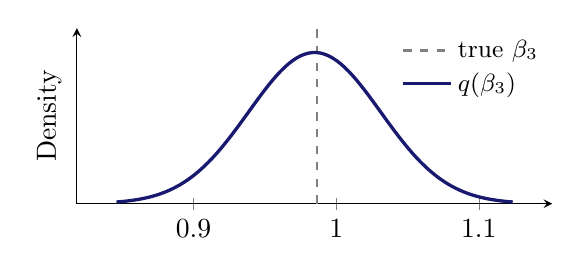
\begin{tikzpicture}

\begin{axis}[
width=3.0in,
height=1.5in,
axis lines=left,
enlarge x limits=0.1,
ylabel={Density},
ylabel near ticks,
ytick=\empty,
legend entries={{true $\beta_3$}, {$q(\beta_3)$}},
legend style={draw=none, at={(1.0,1.0)}, anchor=north east,font=\small},
legend cell align=left,
]
\addplot [thick, dashed, gray]
table {%
0.986584841970366 0
0.986584841970366 10
};
\addplot [very thick, MidnightBlue]
table {%
0.845995739102364 0.0957297390446682
0.848801522092386 0.114607200916625
0.851607305082408 0.136704160356275
0.85441308807243 0.162463704977476
0.857218871062452 0.192369302217613
0.860024654052474 0.226944666945143
0.862830437042496 0.26675280122341
0.865636220032519 0.312394077108754
0.868442003022541 0.364503236581151
0.871247786012563 0.423745190504442
0.874053569002585 0.49080951142261
0.876859351992607 0.566403533441557
0.879665134982629 0.651243996698592
0.882470917972651 0.746047204077195
0.885276700962674 0.851517693758399
0.888082483952696 0.968335472540955
0.890888266942718 1.09714190096996
0.89369404993274 1.23852437126565
0.896499832922762 1.39299997163367
0.899305615912784 1.56099838428567
0.902111398902806 1.74284431767804
0.904917181892829 1.93873982415276
0.907722964882851 2.14874690025235
0.910528747872873 2.37277080631509
0.913334530862895 2.61054457236931
0.916140313852917 2.86161517676441
0.918946096842939 3.12533189051869
0.921751879832961 3.40083727243771
0.924557662822983 3.68706127646313
0.927363445813006 3.98271889272663
0.930169228803028 4.28631168724502
0.93297501179305 4.59613353255179
0.935780794783072 4.91028073392366
0.938586577773094 5.22666665499454
0.941392360763116 5.54304083486749
0.944198143753138 5.85701246933826
0.947003926743161 6.16607800505092
0.949809709733183 6.46765247123206
0.952615492723205 6.75910405327903
0.955421275713227 7.03779130020314
0.958227058703249 7.30110225798107
0.961032841693271 7.54649473724003
0.963838624683293 7.77153685997138
0.966644407673316 7.97394698912894
0.969450190663338 8.15163212928732
0.97225597365336 8.30272389742954
0.975061756643382 8.4256112008756
0.977867539633404 8.5189688238474
0.980673322623426 8.58178121368143
0.983479105613448 8.61336086978972
0.986284888603471 8.61336086978972
0.989090671593493 8.58178121368143
0.991896454583515 8.5189688238474
0.994702237573537 8.4256112008756
0.997508020563559 8.30272389742954
1.00031380355358 8.15163212928732
1.0031195865436 7.97394698912894
1.00592536953363 7.77153685997139
1.00873115252365 7.54649473724004
1.01153693551367 7.30110225798107
1.01434271850369 7.03779130020314
1.01714850149371 6.75910405327903
1.01995428448374 6.46765247123206
1.02276006747376 6.16607800505091
1.02556585046378 5.85701246933825
1.0283716334538 5.54304083486749
1.03117741644382 5.22666665499454
1.03398319943385 4.91028073392366
1.03678898242387 4.5961335325518
1.03959476541389 4.28631168724503
1.04240054840391 3.98271889272663
1.04520633139394 3.68706127646313
1.04801211438396 3.40083727243771
1.05081789737398 3.12533189051869
1.053623680364 2.8616151767644
1.05642946335402 2.6105445723693
1.05923524634405 2.37277080631509
1.06204102933407 2.14874690025235
1.06484681232409 1.93873982415276
1.06765259531411 1.74284431767805
1.07045837830413 1.56099838428568
1.07326416129416 1.39299997163367
1.07606994428418 1.23852437126565
1.0788757272742 1.09714190096996
1.08168151026422 0.96833547254096
1.08448729325425 0.851517693758395
1.08729307624427 0.746047204077192
1.09009885923429 0.651243996698592
1.09290464222431 0.566403533441557
1.09571042521433 0.49080951142261
1.09851620820436 0.423745190504444
1.10132199119438 0.364503236581153
1.1041277741844 0.312394077108753
1.10693355717442 0.26675280122341
1.10973934016444 0.226944666945143
1.11254512315447 0.192369302217614
1.11535090614449 0.162463704977475
1.11815668913451 0.136704160356274
1.12096247212453 0.114607200916625
1.12376825511456 0.0957297390446682
};
\end{axis}

\end{tikzpicture}


\medskip

% This file was created by matplotlib2tikz v0.5.15.
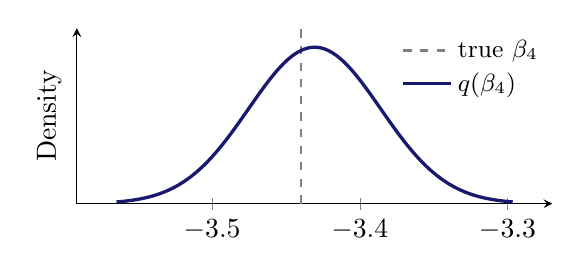
\begin{tikzpicture}

\begin{axis}[
width=3.0in,
height=1.5in,
axis lines=left,
enlarge x limits=0.1,
ylabel={Density},
ylabel near ticks,
ytick=\empty,
legend entries={{true $\beta_4$}, {$q(\beta_4)$}},
legend style={draw=none, at={(1.0,1.0)}, anchor=north east,font=\small},
legend cell align=left,
]
\addplot [thick, dashed, gray]
table {%
-3.43981359557564 0
-3.43981359557564 10
};
\addplot [very thick, MidnightBlue]
table {%
-3.56477700546384 0.0990877818607054
-3.56206630926692 0.118627434247927
-3.55935561307 0.141499518916615
-3.55664491687309 0.168162666270076
-3.55393422067617 0.199117302993386
-3.55122352447925 0.234905515016792
-3.54851282828233 0.276110053596034
-3.54580213208542 0.323352350858125
-3.5430914358885 0.3772894144945
-3.54038073969158 0.43860947935558
-3.53767004349467 0.508026307063375
-3.53495934729775 0.586272043848377
-3.53224865110083 0.674088571920725
-3.52953795490391 0.772217320898544
-3.526827258707 0.881387543010997
-3.52411656251008 1.00230309858413
-3.52140586631316 1.13562784604295
-3.51869517011624 1.28196978236695
-3.51598447391933 1.44186413437105
-3.51327377772241 1.61575565681672
-3.51056308152549 1.80398044840246
-3.50785238532857 2.00674764913621
-3.50514168913166 2.2241214302979
-3.50243099293474 2.45600372891326
-3.49972029673782 2.70211821014031
-3.49700960054091 2.96199596106921
-3.49429890434399 3.23496342620889
-3.49158820814707 3.52013308672892
-3.48887751195015 3.81639736110385
-3.48616681575324 4.12242616341894
-3.48345611955632 4.43666849707539
-3.4807454233594 4.75735838644311
-3.47803472716248 5.08252535829877
-3.47532403096557 5.41000958048226
-3.47261333476865 5.73748164960578
-3.46990263857173 6.06246689596034
-3.46719194237481 6.38237394562925
-3.4644812461779 6.6945271512885
-3.46177054998098 6.99620237857971
-3.45905985378406 7.28466551872985
-3.45634915758715 7.55721299463653
-3.45363846139023 7.81121344107799
-3.45092776519331 8.04414967373889
-3.44821706899639 8.2536600194738
-3.44550637279948 8.43757806399793
-3.44279567660256 8.59396988447118
-3.44008498040564 8.72116787371497
-3.43737428420872 8.81780032954718
-3.43466358801181 8.88281607537638
-3.43195289181489 8.9155034942174
-3.42924219561797 8.9155034942174
-3.42653149942105 8.88281607537638
-3.42382080322414 8.81780032954718
-3.42111010702722 8.72116787371497
-3.4183994108303 8.59396988447118
-3.41568871463339 8.43757806399793
-3.41297801843647 8.2536600194738
-3.41026732223955 8.04414967373889
-3.40755662604263 7.81121344107799
-3.40484592984572 7.55721299463653
-3.4021352336488 7.2846655187298
-3.39942453745188 6.99620237857971
-3.39671384125496 6.6945271512885
-3.39400314505805 6.38237394562925
-3.39129244886113 6.06246689596034
-3.38858175266421 5.73748164960578
-3.38587105646729 5.41000958048226
-3.38316036027038 5.08252535829877
-3.38044966407346 4.75735838644311
-3.37773896787654 4.43666849707539
-3.37502827167963 4.12242616341894
-3.37231757548271 3.81639736110385
-3.36960687928579 3.52013308672892
-3.36689618308887 3.23496342620889
-3.36418548689196 2.96199596106921
-3.36147479069504 2.70211821014031
-3.35876409449812 2.45600372891326
-3.3560533983012 2.2241214302979
-3.35334270210429 2.00674764913621
-3.35063200590737 1.80398044840246
-3.34792130971045 1.61575565681672
-3.34521061351353 1.44186413437105
-3.34249991731662 1.28196978236695
-3.3397892211197 1.13562784604295
-3.33707852492278 1.00230309858413
-3.33436782872587 0.881387543010997
-3.33165713252895 0.772217320898544
-3.32894643633203 0.674088571920725
-3.32623574013511 0.586272043848377
-3.3235250439382 0.508026307063375
-3.32081434774128 0.43860947935558
-3.31810365154436 0.3772894144945
-3.31539295534744 0.323352350858125
-3.31268225915053 0.276110053596027
-3.30997156295361 0.234905515016792
-3.30726086675669 0.199117302993386
-3.30455017055977 0.168162666270076
-3.30183947436286 0.141499518916615
-3.29912877816594 0.118627434247927
-3.29641808196902 0.0990877818607054
};
\end{axis}

\end{tikzpicture}

\caption{Visualization of the inferred marginal posteriors for Bayesian linear
regression. The gray bars indicate the simulated ``true'' value for each
component of the coefficient vector.}
\label{fig:supervised-betas}
\end{figure}

\subsubsection{Criticism}

A standard evaluation in regression is to calculate point-based evaluations on
held-out ``testing'' data. We do this first by forming the posterior predictive
distribution.
\begin{lstlisting}
y_post = Normal(mu=ed.dot(X, qw.mean()) + qb.mean(), sigma=tf.ones(N))
\end{lstlisting}

With this we can evaluate various point-based quantities using the posterior
predictive.
\begin{lstlisting}
print(ed.evaluate('mean_squared_error', data={X: X_test, y_post: y_test}))
> 0.012107

print(ed.evaluate('mean_absolute_error', data={X: X_test, y_post: y_test}))
> 0.0867875
\end{lstlisting}

The trained model makes predictions with low mean squared error
(relative to the magnitude of the output).

Edward supports another class of criticism techniques called
\glspl{PPC}.
The simplest \gls{PPC} works by applying a test statistic on new data
generated from the posterior predictive, such as
$T(\mathbf{x}_\text{new}) = \max(\mathbf{x}_\text{new})$.
Applying $T(\mathbf{x}_\text{new})$ to
new data over many data replications induces a distribution of the test
statistic, $\textsc{ppd}(T)$. We compare
this distribution to the test statistic applied to the original dataset
$T(\mathbf{x})$.

Calculating \glspl{PPC} in Edward is straightforward.
\begin{lstlisting}
def T(xs, zs):
  return tf.reduce_max(xs[y_post])

ppc_max = ed.ppc(T, data={X: X_train, y_post: y_train})
\end{lstlisting}
This calculates the test statistic on both the original dataset as well as on
data replications generated from teh posterior predictive distribution.
Figure \ref{fig:supervised-ppc} shows three visualizations of different \glspl
{PPC}; the
plotted posterior predictive distributions are kernel density estimates from
$N=500$ data replications.


\begin{figure}[htb]
\centering
% This file was created by matplotlib2tikz v0.5.15.
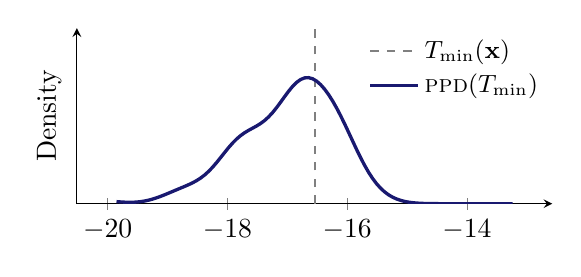
\begin{tikzpicture}

\begin{axis}[
width=3.0in,
height=1.5in,
axis lines=left,
enlarge x limits=0.1,
ylabel={Density},
ylabel near ticks,
ytick=\empty,
legend entries={{$T_\text{min}(\mathbf{x})$}, {$\textsc{ppd}(T_\text{min})$}},
legend style={draw=none, at={(1.0,1.0)}, anchor=north east,font=\small},
legend cell align=left,
]
\addplot [thick, dashed, gray]
table {%
-16.5441242364738 0
-16.5441242364738 0.7
};
\addplot [very thick, MidnightBlue]
table {%
-13.2352993891791 5.05219293070858e-13
-13.3021443355891 2.05825068882034e-12
-13.3689892819991 8.038769482291e-12
-13.4358342284091 3.01002711420105e-11
-13.5026791748191 1.08058842088904e-10
-13.5695241212291 3.71948112238135e-10
-13.6363690676391 1.22761967091541e-09
-13.703214014049 3.88541167689218e-09
-13.770058960459 1.17934327544065e-08
-13.836903906869 3.43335601433984e-08
-13.903748853279 9.58797378067529e-08
-13.970593799689 2.56878942376166e-07
-14.037438746099 6.60390007322067e-07
-14.104283692509 1.62942503466722e-06
-14.171128638919 3.85957766174606e-06
-14.237973585329 8.77906132307628e-06
-14.304818531739 1.91830211203899e-05
-14.371663478149 4.02843232474005e-05
-14.438508424559 8.13454163652436e-05
-14.505353370969 0.000158045340654349
-14.572198317379 0.000295671862401375
-14.639043263789 0.000533101503267019
-14.705888210199 0.000927356629459576
-14.772733156609 0.00155836143375224
-14.839578103019 0.0025334377221303
-14.906423049429 0.00399115809416706
-14.973267995839 0.00610441074410488
-15.040112942249 0.00908280448773802
-15.1069578886589 0.0131746032563921
-15.1738028350689 0.0186679352142648
-15.2406477814789 0.0258899291011952
-15.3074927278889 0.0352009076844701
-15.3743376742989 0.0469795037322437
-15.4411826207089 0.061594575989866
-15.5080275671189 0.0793620014551975
-15.5748725135289 0.100488999535781
-15.6417174599389 0.125014606287185
-15.7085624063489 0.152760090791724
-15.7754073527589 0.183304841215112
-15.8422522991689 0.215999631691617
-15.9090972455789 0.250020225923821
-15.9759421919889 0.284452402130418
-16.0427871383989 0.318388874103353
-16.1096320848089 0.351013519104097
-16.1764770312189 0.38165129488892
-16.2433219776289 0.409772728951764
-16.3101669240389 0.434956507091933
-16.3770118704489 0.456827556412376
-16.4438568168589 0.474996523312243
-16.5107017632689 0.489026959953148
-16.5775467096788 0.498448653141407
-16.6443916560888 0.502821529311249
-16.7112366024988 0.501838316951246
-16.7780815489088 0.495440274532375
-16.8449264953188 0.483913062864297
-16.9117714417288 0.467931894223707
-16.9786163881388 0.448536362773748
-17.0454613345488 0.427032755011925
-17.1123062809588 0.404839873801779
-17.1791512273688 0.383307916393971
-17.2459961737788 0.363545023299929
-17.3128411201888 0.346282271150708
-17.3796860665988 0.331797694426288
-17.4465310130088 0.319907513582849
-17.5133759594188 0.31002177463391
-17.5802209058288 0.301253806284686
-17.6470658522388 0.292567919168833
-17.7139107986488 0.282946187091122
-17.7807557450588 0.271552000520565
-17.8476006914688 0.257865922265467
-17.9144456378788 0.241770195825571
-17.9812905842888 0.223564258665736
-18.0481355306987 0.20390550471423
-18.1149804771087 0.183685389894948
-18.1818254235187 0.163866398952204
-18.2486703699287 0.145315174953473
-18.3155153163387 0.128667506515823
-18.3823602627487 0.114251399827959
-18.4492052091587 0.102078285357883
-18.5160501555687 0.0918949883808782
-18.5828951019787 0.0832759071210482
-18.6497400483887 0.0757292467898767
-18.7165849947987 0.0687933906826522
-18.7834299412087 0.0621071419943456
-18.8502748876187 0.0554470682033875
-18.9171198340287 0.0487334112562898
-18.9839647804387 0.0420113379764541
-19.0508097268487 0.0354165758884345
-19.1176546732587 0.0291345116183055
-19.1844996196687 0.023360572096513
-19.2513445660787 0.0182677812430854
-19.3181895124887 0.0139850418440157
-19.3850344588987 0.0105870889772692
-19.4518794053086 0.00809451956674418
-19.5187243517186 0.0064803640817207
-19.5855692981286 0.0056788992121118
-19.6524142445386 0.00559309392058319
-19.7192591909486 0.00609902076360903
-19.7861041373586 0.00704802346396004
-19.8529490837686 0.00826940904339173
};
\end{axis}

\end{tikzpicture}

% This file was created by matplotlib2tikz v0.5.15.
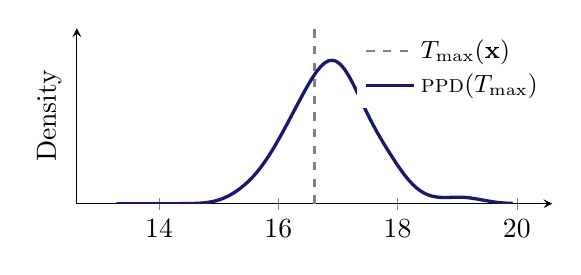
\begin{tikzpicture}

\begin{axis}[
width=3.0in,
height=1.5in,
axis lines=left,
enlarge x limits=0.1,
ylabel={Density},
ylabel near ticks,
ytick=\empty,
legend entries={{$T_\text{max}(\mathbf{x})$}, {$\textsc{ppd}(T_\text{max})$}},
legend style={draw=none, at={(1.0,1.0)}, anchor=north east,font=\small},
legend cell align=left,
]
\addplot [thick, dashed, gray]
table {%
16.6090179263646 0
16.6090179263646 0.7
};
\addplot [very thick, MidnightBlue]
table {%
13.2872143410917 5.88907908239748e-12
13.3543214842285 2.30682665294251e-11
13.4214286273653 8.65546789880128e-11
13.4885357705022 3.1109455968171e-10
13.555642913639 1.0711268332124e-09
13.6227500567758 3.53312245190288e-09
13.6898571999126 1.11653193225071e-08
13.7569643430495 3.3807003201652e-08
13.8240714861863 9.80837688954409e-08
13.8911786293231 2.72695790757017e-07
13.9582857724599 7.26592725735176e-07
14.0253929155968 1.85558514831365e-06
14.0925000587336 4.54255547295968e-06
14.1596072018704 1.06612705924626e-05
14.2267143450072 2.39925316082358e-05
14.2938214881441 5.17823461453552e-05
14.3609286312809 0.0001072061804853
14.4280357744177 0.000212961676966936
14.4951429175546 0.000406031146985154
14.5622500606914 0.000743282168077874
14.6293572038282 0.00130701292524395
14.696464346965 0.0022089106794077
14.7635714901019 0.00359042894948312
14.8306786332387 0.00561765895060876
14.8977857763755 0.00846970343296913
14.9648929195123 0.0123214421175529
15.0320000626492 0.0173240355812697
15.099107205786 0.0235886564903373
15.1662143489228 0.031179576611542
15.2333214920596 0.0401209248561671
15.3004286351965 0.0504171026374971
15.3675357783333 0.0620812265945392
15.4346429214701 0.0751613769177472
15.501750064607 0.0897533274782765
15.5688572077438 0.105992124712952
15.6359643508806 0.124022507817905
15.7030714940174 0.143956727359728
15.7701786371543 0.165833949246076
15.8372857802911 0.189595328748755
15.9043929234279 0.215082843128724
15.9715000665647 0.242060737082459
16.0386072097016 0.270250050733925
16.1057143528384 0.299362541219018
16.1728214959752 0.32912144615983
16.239928639112 0.359261610668238
16.3070357822489 0.389507960577613
16.3741429253857 0.419537018754109
16.4412500685225 0.448930257716725
16.5083572116594 0.477130658103593
16.5754643547962 0.503415058089259
16.642571497933 0.526894349720654
16.7096786410698 0.546550574825499
16.7767857842067 0.561314151873328
16.8438929273435 0.570176434087392
16.9110000704803 0.572324061977174
16.9781072136171 0.567274001154524
17.045214356754 0.554983501388671
17.1123214998908 0.535908974244704
17.1794286430276 0.51099320138505
17.2465357861644 0.481571955357454
17.3136429293013 0.449208111466936
17.3807500724381 0.415480326874349
17.4478572155749 0.381768753084954
17.5149643587118 0.349085826732023
17.5820715018486 0.317991959931194
17.6491786449854 0.28861464804705
17.7162857881222 0.260761178662522
17.7833929312591 0.234089181792312
17.8505000743959 0.208284730263077
17.9176072175327 0.183199427299166
17.9847143606695 0.15891462704636
18.0518215038064 0.135725953354043
18.1189286469432 0.114065475069874
18.18603579008 0.0943943177157276
18.2531429332168 0.0771011977617766
18.3202500763537 0.062433366545238
18.3873572194905 0.0504707003030209
18.4544643626273 0.0411377501446338
18.5215715057642 0.0342380739875309
18.588678648901 0.0294928336595045
18.6557857920378 0.0265706969754408
18.7228929351746 0.025105076939142
18.7900000783115 0.0247032169000523
18.8571072214483 0.0249560346592097
18.9242143645851 0.0254566143186622
18.9913215077219 0.0258298999634965
19.0584286508588 0.0257693361585591
19.1255357939956 0.0250711059829185
19.1926429371324 0.0236554243582867
19.2597500802692 0.0215674372259132
19.3268572234061 0.0189562594568207
19.3939643665429 0.0160371232920431
19.4610715096797 0.0130461174367693
19.5281786528165 0.0101981696569966
19.5952857959534 0.00765675999972511
19.6623929390902 0.00551954424981433
19.729500082227 0.0038193648300069
19.7966072253639 0.00253657419000109
19.8637143685007 0.00161701386050297
19.9308215116375 0.000990349592964849
};
\end{axis}

\end{tikzpicture}


\medskip

% This file was created by matplotlib2tikz v0.5.15.
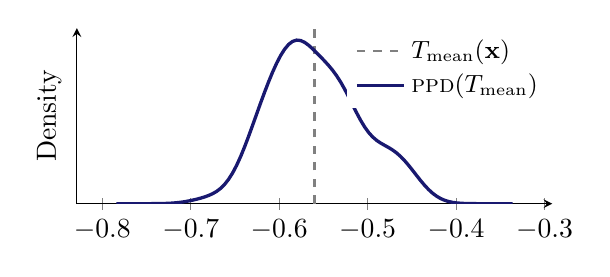
\begin{tikzpicture}

\begin{axis}[
width=3.0in,
height=1.5in,
axis lines=left,
enlarge x limits=0.1,
ylabel={Density},
ylabel near ticks,
ytick=\empty,
legend entries={{$T_\text{mean}(\mathbf{x})$}, {$\textsc{ppd}(T_\text{mean})$}},
legend style={draw=none, at={(1.0,1.0)}, anchor=north east,font=\small},
legend cell align=left,
]
\addplot [thick, dashed, gray]
table {%
-0.559917133751622 0
-0.559917133751622 8
};
\addplot [very thick, MidnightBlue]
table {%
-0.335950280250973 1.31826193247141e-07
-0.340474863149976 4.40417152547664e-07
-0.344999446048979 1.40051041254e-06
-0.349524028947982 4.23967782308379e-06
-0.354048611846985 1.22201874775514e-05
-0.358573194745988 3.3543340518437e-05
-0.363097777644991 8.77032514473706e-05
-0.367622360543994 0.000218483251802879
-0.372146943442997 0.000518731692386615
-0.376671526342 0.0011741899396429
-0.381196109241003 0.00253499069727522
-0.385720692140006 0.00522221230327025
-0.390245275039009 0.0102707121664167
-0.394769857938012 0.019296407749699
-0.399294440837015 0.0346563621203797
-0.403819023736018 0.0595475810788749
-0.408343606635021 0.097974212874276
-0.412868189534024 0.154514642298559
-0.417392772433027 0.233849438781403
-0.42191735533203 0.34006905738358
-0.426441938231033 0.475853928256519
-0.430966521130036 0.641684585993456
-0.435491104029039 0.835268781763808
-0.440015686928042 1.05135004425149
-0.444540269827045 1.28199255463699
-0.449064852726048 1.51734460173359
-0.453589435625051 1.74679787721112
-0.458114018524054 1.96040229159795
-0.462638601423057 2.15036528409097
-0.46716318432206 2.31244527582332
-0.471687767221063 2.4470278702521
-0.476212350120066 2.55965637579346
-0.480736933019069 2.66080216636917
-0.485261515918072 2.76473802573947
-0.489786098817075 2.88753333272035
-0.494310681716078 3.04440269712009
-0.498835264615081 3.24685395853415
-0.503359847514084 3.50022588193761
-0.507884430413087 3.80221894074062
-0.51240901331209 4.14287445862823
-0.516933596211093 4.5061614945854
-0.521458179110096 4.87294490313373
-0.525982762009099 5.22472548384073
-0.530507344908102 5.54727438361957
-0.535031927807105 5.83322641691359
-0.539556510706108 6.08290049624787
-0.544081093605111 6.30305460135884
-0.548605676504114 6.50385157623385
-0.553130259403117 6.69484690038952
-0.55765484230212 6.88113690254679
-0.562179425201123 7.06080036809693
-0.566704008100126 7.22440154665388
-0.571228590999129 7.35669463994601
-0.575753173898132 7.43998095855344
-0.580277756797135 7.4580631623682
-0.584802339696138 7.39960494788908
-0.589326922595141 7.25998696678778
-0.593851505494144 7.04132844890974
-0.598376088393147 6.75097937727867
-0.60290067129215 6.39923484102435
-0.607425254191153 5.99714012155065
-0.611949837090156 5.55505271572972
-0.616474419989159 5.08223599892622
-0.620999002888162 4.58734843736424
-0.625523585787165 4.07939787597822
-0.630048168686168 3.56862012110047
-0.634572751585171 3.06681792580805
-0.639097334484174 2.58691662728942
-0.643621917383177 2.14178028998728
-0.64814650028218 1.74259488341976
-0.652671083181183 1.39727785944853
-0.657195666080186 1.10936936894104
-0.661720248979189 0.87770989538598
-0.666244831878192 0.696974855475188
-0.670769414777195 0.558903275250046
-0.675293997676198 0.453895730432368
-0.679818580575201 0.372601409041363
-0.684343163474204 0.307163343307327
-0.688867746373207 0.251916462815002
-0.69339232927221 0.203493603930414
-0.697916912171213 0.160444778103095
-0.702441495070216 0.12257535509535
-0.706966077969219 0.0902362521484529
-0.711490660868222 0.0637553138982275
-0.716015243767225 0.0431095405530541
-0.720539826666228 0.0278410195212284
-0.725064409565231 0.0171492513326823
-0.729588992464234 0.0100653399100707
-0.734113575363237 0.00562517074090984
-0.73863815826224 0.00299195464813669
-0.743162741161243 0.00151403282434576
-0.747687324060246 0.000728732711755793
-0.752211906959249 0.000333561443670076
-0.756736489858252 0.000145178214655598
-0.761261072757255 6.00764012086311e-05
-0.765785655656258 2.363486586849e-05
-0.770310238555261 8.83948805819745e-06
-0.774834821454264 3.14274855194534e-06
-0.779359404353267 1.0621571788719e-06
-0.78388398725227 3.41236740996593e-07
};
\end{axis}

\end{tikzpicture}

\glsreset{PPC}
\caption{Examples of \glspl{PPC} for Bayesian linear regression. }
\label{fig:supervised-ppc}
\end{figure}





\subsection{Logistic and Neural Network Classification}

In supervised learning, the task is to infer hidden structure from
labeled data, comprised of training examples $\{(x_n, y_n)\}$.
Classification means the output $y$ takes discrete values.


\subsubsection{Data}

We study a two-dimensional simulated dataset with a nonlinear decision
boundary. We simulate $100$ datapoints using the following snippet.
\begin{lstlisting}
from scipy.stats import logistic

N = 100  # number of data points
D = 2  # number of features

px1 = np.linspace(-3, 3, 50)
px2 = np.linspace(-3, 3, 50)
px1_m, px2_m = np.mgrid[-3:3:50j, -3:3:50j]

xeval = np.vstack((px1_m.flatten(), px2_m.flatten())).T
x_viz = tf.constant(np.array(xeval, dtype='float32'))

def build_toy_dataset(N):
  x = xeval[np.random.randint(xeval.shape[0],size=N), :]
  y = bernoulli.rvs(p=logistic.cdf( 5 * x[:, 0]**2 + 5 * x[:, 1]**3 ))
  return x, y

x_train, y_train = build_toy_dataset(N)
\end{lstlisting}

Figure\nobreakspace \ref{fig:lr_data} shows the data, colored by label. The red point near the
origin makes this a challenging dataset for classification models that assume a
linear decision boundary.
\begin{figure}[!htbp]
\centering
\includegraphics[width=2.5in]{images/lr_data.pdf}
\caption{Simulated data for classification. Positive and negative measurements
colored by label.}
\label{fig:lr_data}
\end{figure}


\subsubsection{Model: Bayesian Logistic Regression}

We begin with a popular classification model: logistic regression. This model
relates outputs $y\in\{0,1\}$, also known as the response, given
a vector of inputs $\mathbf{x}\in\mathbb{R}^D$, also known as the features or
covariates. The model assumes a latent linear relationship between these two random
variables \citep{gelman2013bayesian}.

The likelihood of each datapoint is a Bernoulli with probability
\begin{align*}
\Pr(y_n=1)
  &=
  \text{logistic}
  \left(
  \mathbf{x}^\top \mathbf{w} + b
  \right).
\end{align*}
We posit priors on the latent variables $\mathbf{w}$ and $b$ as
\begin{align*}
  p(\mathbf{w})
  &=
  \text{Normal}(\mathbf{w} \mid \mathbf{0}, \sigma_w^2\mathbf{I}),
  \\
  p(b)
  &=
  \text{Normal}(b \mid 0, \sigma_b^2).
\end{align*}

This model is
easy to specify in Edward's native language.

\begin{lstlisting}
W = Normal(mu=tf.zeros(D), sigma=tf.ones(D))
b = Normal(mu=tf.zeros(1), sigma=tf.ones(1))

x = tf.cast(x_train, dtype=tf.float32)
y = Bernoulli(logits=(ed.dot(x, W) + b))
\end{lstlisting}


\subsubsection{Inference}

Here, we perform variational inference. Define the variational model to be a
fully factorized normal
\begin{lstlisting}
qW = Normal(mu=tf.Variable(tf.random_normal([D])),
            sigma=tf.nn.softplus(tf.Variable(tf.random_normal([D]))))
qb = Normal(mu=tf.Variable(tf.random_normal([1])),
            sigma=tf.nn.softplus(tf.Variable(tf.random_normal([1]))))
\end{lstlisting}

Run variational inference with the Kullback-Leibler divergence for $1000$ iterations.
\begin{lstlisting}
inference = ed.KLqp({W: qW, b: qb}, data={y: y_train})
inference.run(n_iter=1000, n_print=100, n_samples=5)
\end{lstlisting}
In this case
\texttt{KLqp} defaults to minimizing the
$\text{KL}(q\|p)$ divergence measure using the reparameterization
gradient.


\subsubsection{Criticism}

The first thing to look at are point-wise evaluations on the training dataset.

First form a plug-in estimate of the posterior predictive distribution.
\begin{lstlisting}
y_post = ed.copy(y, {W: qW.mean(), b: qb.mean()})
\end{lstlisting}

Then evaluate predictive accuracy
\begin{lstlisting}
print('Plugin estimate of posterior predictive log accuracy on training data:')
print(ed.evaluate('log_lik', data={x: x_train, y_post: y_train}))
> -3.12

print('Binary accuracy on training data:')
print(ed.evaluate('binary_accuracy', data={x: x_train, y_post: y_train}))
> 0.71
\end{lstlisting}

Figure\nobreakspace \ref {fig:lr_linear} shows the posterior label probability evaluated on a grid.
As expected, logistic regression attempts to fit a linear boundary between the
two label classes. Can a non-linear model do better?
\begin{figure}[!htb]
\centering
\includegraphics[width=2.5in]{images/lr_linear.pdf}
\caption{Logistic regression struggles to separate the measurements.}
\label{fig:lr_linear}
\end{figure}

\subsubsection{Model: Bayesian Neural Network Classification}

Consider parameterizing the label probability using a neural network; this
model is not limited to a linear relationship to the inputs $\mathbf{x}$, as in
logistic regression.

The model posits a likelihood for each observation $(\mathbf{x}_n,
y_n)$ as
\begin{align*}
\Pr(y_n=1)
  &=
  \text{logistic}
  \left(
  \text{NN}(\mathbf{x}_n \;;\; \mathbf{z})
  \right),
\end{align*}
where NN is a neural network and the latent random variable $\mathbf{z}$
contains its weights and biases.

We can specify a Bayesian neural network in Edward as follows. Here we specify a
fully connected two-layer network with two nodes in each layer; we posit
standard normal priors on all weights and biases.
\begin{lstlisting}
def neural_network(x, W_0, W_1, W_2, b_0, b_1, b_2):
    h = tf.nn.tanh(tf.matmul(x, W_0) + b_0)
    h = tf.nn.tanh(tf.matmul(h, W_1) + b_1)
    h = tf.matmul(h, W_2) + b_2
    return tf.reshape(h, [-1])

H = 2  # number of hidden units in each layer

W_0 = Normal(mu=tf.zeros([D, H]), sigma=tf.ones([D, H]))
W_1 = Normal(mu=tf.zeros([H, H]), sigma=tf.ones([H, H]))
W_2 = Normal(mu=tf.zeros([H, 1]), sigma=tf.ones([H, 1]))
b_0 = Normal(mu=tf.zeros(H), sigma=tf.ones(H))
b_1 = Normal(mu=tf.zeros(H), sigma=tf.ones(H))
b_2 = Normal(mu=tf.zeros(1), sigma=tf.ones(1))

x = tf.cast(x_train, dtype=tf.float32)
y = Bernoulli(logits=neural_network(x, W_0, W_1, W_2, b_0, b_1, b_2))
\end{lstlisting}

\subsubsection{Inference}

Similar to the above, we perform variational inference. Define the variational
model to be a fully factorized normal over all latent variables
\begin{lstlisting}
qW_0 = Normal(mu=tf.Variable(tf.random_normal([D, H])),
              sigma=tf.nn.softplus(tf.Variable(tf.random_normal([D, H]))))
qW_1 = Normal(mu=tf.Variable(tf.random_normal([H, H])),
              sigma=tf.nn.softplus(tf.Variable(tf.random_normal([H, H]))))
qW_2 = Normal(mu=tf.Variable(tf.random_normal([H, 1])),
              sigma=tf.nn.softplus(tf.Variable(tf.random_normal([H, 1]))))
qb_0 = Normal(mu=tf.Variable(tf.random_normal([H])),
              sigma=tf.nn.softplus(tf.Variable(tf.random_normal([H]))))
qb_1 = Normal(mu=tf.Variable(tf.random_normal([H])),
              sigma=tf.nn.softplus(tf.Variable(tf.random_normal([H]))))
qb_2 = Normal(mu=tf.Variable(tf.random_normal([1])),
              sigma=tf.nn.softplus(tf.Variable(tf.random_normal([1]))))
\end{lstlisting}

Run variational inference for $1000$ iterations.
\begin{lstlisting}
inference = ed.KLqp({W_0: qW_0, b_0: qb_0,
                     W_1: qW_1, b_1: qb_1,
                     W_2: qW_2, b_2: qb_2}, data={y: y_train})
inference.run(n_iter=1000, n_print=100, n_samples=5)
\end{lstlisting}

\subsubsection{Criticism}

Again, we form a plug-in estimate of the posterior predictive distribution.
\begin{lstlisting}
y_post = ed.copy(y, {W_0: qW_0.mean(), b_0: qb_0.mean(),
                     W_1: qW_1.mean(), b_1: qb_1.mean(),
                     W_2: qW_2.mean(), b_1: qb_2.mean()})
\end{lstlisting}

Both predictive accuracy metrics look better.
\begin{lstlisting}
print('Plugin estimate of posterior predictive log accuracy on training data:')
print(ed.evaluate('log_lik', data={x: x_train, y_post: y_train}))
> -0.170941

print('Binary accuracy on training data:')
print(ed.evaluate('binary_accuracy', data={x: x_train, y_post: y_train}))
> 0.81
\end{lstlisting}

Figure\nobreakspace \ref{fig:lr_nn} shows the posterior label probability evaluated on a grid.
The neural network has captured the nonlinear decision boundary between the two
label classes.
\begin{figure}[!htb]
\centering
\includegraphics[width=2.5in]{images/lr_nn.pdf}
\caption{A Bayesian neural network does a better job of separating the two
label classes.}
\label{fig:lr_nn}
\end{figure}


\clearpage
\section{Acknowledgments}
Edward has benefited enormously from the helpful feedback and advice
of many individuals: Jaan Altosaar, Eugene Brevdo, Allison Chaney,
Joshua Dillon, Matthew Hoffman, Kevin Murphy, Rajesh Ranganath, Rif
Saurous, and other members of the Blei Lab, Google Brain, and Google
Research.
This work is supported by NSF IIS-1247664, ONR N00014-11-1-0651,
DARPA FA8750-14-2-0009, DARPA N66001-15-C-4032, Adobe, Google, NSERC
PGS-D, and the Sloan Foundation.

\clearpage
\bibliographystyle{apalike}
\bibliography{bib}

\end{document}
